\chapter{Discussion}\label{ch:discussion}
\section{Introduction}

In the preceding chapters, I laid out an analysis of Eastern Indonesian \textsc{multi-verb construction}s based on different perspectives. In Chapter \ref{ch:gram}, I investigated the morphosyntactic properties of MVCs that are accessible from published data sources. I focused on three factors: referential interaction between the participating verbs (argument sharing), inflection patterns (addressed in terms of headedness features), and placement options (contiguity) of the verbs. In Chapter \ref{ch:sem}, I then turned to a semantic perspective on MVCs, and proposed two semantic frameworks that may help categorise MVCs into types. By applying a lexical decomposition model and Davidsonian event arguments, I argued for a set of four techniques of verbal interaction underlying the wealth of MVCs in Eastern Indonesia: \textsc{merging}, \textsc{modification}, \textsc{staging} proper, and \textsc{free juxtaposition}. These four techniques were argued to each constitute a major family of MVCs. In Chapter \ref{ch:constructions}, I combined the findings from Chapter \ref{ch:gram} with a theory of MVC formation on different conceptual levels from Chapter \ref{ch:sem} in order to arrive at a classification of MVCs. The four basic constructional families were further elaborated, and furnished with examples and data on their occurrence and distribution in the area. \textsc{Component-relating construction}s were defined as those constructions that merge part of their sublexical components. Modifying constructions comprise a matrix verb that is complemented by a modifier verb adding specific semantic content. Unlike the merging scenario, modifying constructions do not consist of verbs that share sublexical features. Staging proper was claimed to underly \textsc{stage-relating construction}s that are composed of two independent event stages, each licensed by an event argument. Finally, a fourth family of constructions was identified that also aligns more than one \textsc{event stage}, albeit without signs of producing a coherent unit on different levels (that is, lacking a monoclausal reading, a coherent prosodic phrasing, and so on).

In the present chapter, I will pick up some of the loose threads from the preceding discussion, and work out at least to some extent how these findings can be interpreted and framed into a more coherent picture. As has become obvious throughout this book, a literature survey of published data is quite limited in various ways. Published primary data deny the analyst the possibility of thoroughly testing many of the claims raised in the serialisation literature. The nature of the current study prevented me from filling this lacuna by simply adding more data to my analysis; as a result, the findings gained from the EI sample remain to be explored further. Therefore, the discussion in the following sections should be understood as a collection of suggestive pieces of evidence hopefully stimulating further scrutiny. I will specifically focus on properties and patterns that can be addressed through my data annotation.

In §\ref{sec:distribution} I will review the EI sample with regard to the question of what the data can tell us about the distribution and diversity of MVCs across the area. I will try to show that the number of different constructions is only one possible indicator for the amount of MVC use per language. In order to account for the frequency of MVC use, a standardised sample would be needed for all languages. As this is beyond the scope of this book, I will take the number of attested instances as a preliminary measure of MVC diversity in a given language.

The following section §\ref{sec:hierarchy} then turns to another factor that may reveal the extent to which a given language utilises MVCs. I have already discussed in Chapter \ref{ch:theory} that some MVCs can be dissected into what I call \textsc{stacked MVCs}: more than one MVC nested into another. Taking this hypothesis seriously would mean rethinking the issue of hierarchies in MVCs. In this section, I will explore briefly what it means to postulate hidden hierarchies, and how the issue could be approached theoretically. I will then explore the EI sample by computing how many MVCs per language are in fact complex, in the sense that they contain another MVC at a lower level.

In §\ref{sec:profile_use}, I will compare the results obtained from the previous two sections, and propose a broad typology of MVC use across EI. I will distinguish between four different usage profiles. Mapping these profiles on the EI languages will show that languages from all four subareas vary considerably in the extent to which MVCs pervade their grammatical system. Despite this variation, two major core areas of MVC use can be identified.

§\ref{sec:discourse} shifts the perspective back to an issue that I raised before in the discussion of prosodic properties of MVCs (chapter \ref{ch:theory}). It is far from clear, and actually quite improbable, that the syntactic boundaries of MVCs always match with prosodic boundaries. The criterion of coherent, or even `monoclausal', intonation units for MVCs is thus hardly sustainable, and would probably not be borne out by a more comprehensive investigation into natural speech data. Although it is beyond the scope of this book to carry out such an analysis, §\ref{sec:discourse} will nonetheless gather evidence from some of the languages in order to point out some remarkable pieces of evidence. Findings from the two corpus languages Waima'a and Wooi will shed new light on the formation of at least some of the MVC types attested in Eastern Indonesia. Specifically, I will suggest that stage-relating MVCs might rather arise from strategies of discourse development than from concrete grammatical constructions \textit{sensu stricto}.

\section{Distribution and diversity of MVCs} \label{sec:distribution}

As the discussion in §\ref{sec:dist_types} and later sections in Chapter \ref{ch:constructions} has shown, neither the four constructional families CREL, MOD, SREL, and FJUX, nor their specific constructions occur in an even distribution across the EI area. Rather, what the data show is a complex picture of different languages attesting to different constructions in different numbers. What the findings suggest is that while genetic affiliation does not significantly influence the availability of MVCs in a given language, the different subareas do show different preferences in MVC use. The figures for constructions per subarea, given in Chapter \ref{ch:constructions}, are repeated here for convenience. Although the overall distribution of the constructions shows little variation across EI, some constructions are prevalent in some subareas and less so in others. It is the Sulawesi subarea that deviates the most. There are constructions from the component-relating and the stage-relating family that are hardly attested in Sulawesi, or not at all. What is particularily striking in the Sulawesi data is that stage-relating constructions are more or less confined to \textsc{motion-to-action} (the predominant MVC across all of EI), and, to a weaker degree, to resultatives. However, this evidence is not sufficient in order to claim that the Sulawesi languages show an overall lack of MVC use. As we shall see below, the Sulawesi languages compensate for the lack of CREL and SREL constructions with a wealth of modifying constructions, though their use within Sulawesi is by no means evenly distributed. If any subset of EI languages may be qualified as constituting a peripheral group, it is the northern Sulawesi languages Pendau and Tajio that fit this characterisation the most, as they lack many of the constructions that abound in other parts of Eastern Indonesia.

\begin{sidewaysfigure}
\begin{minipage}{1.0\textwidth}
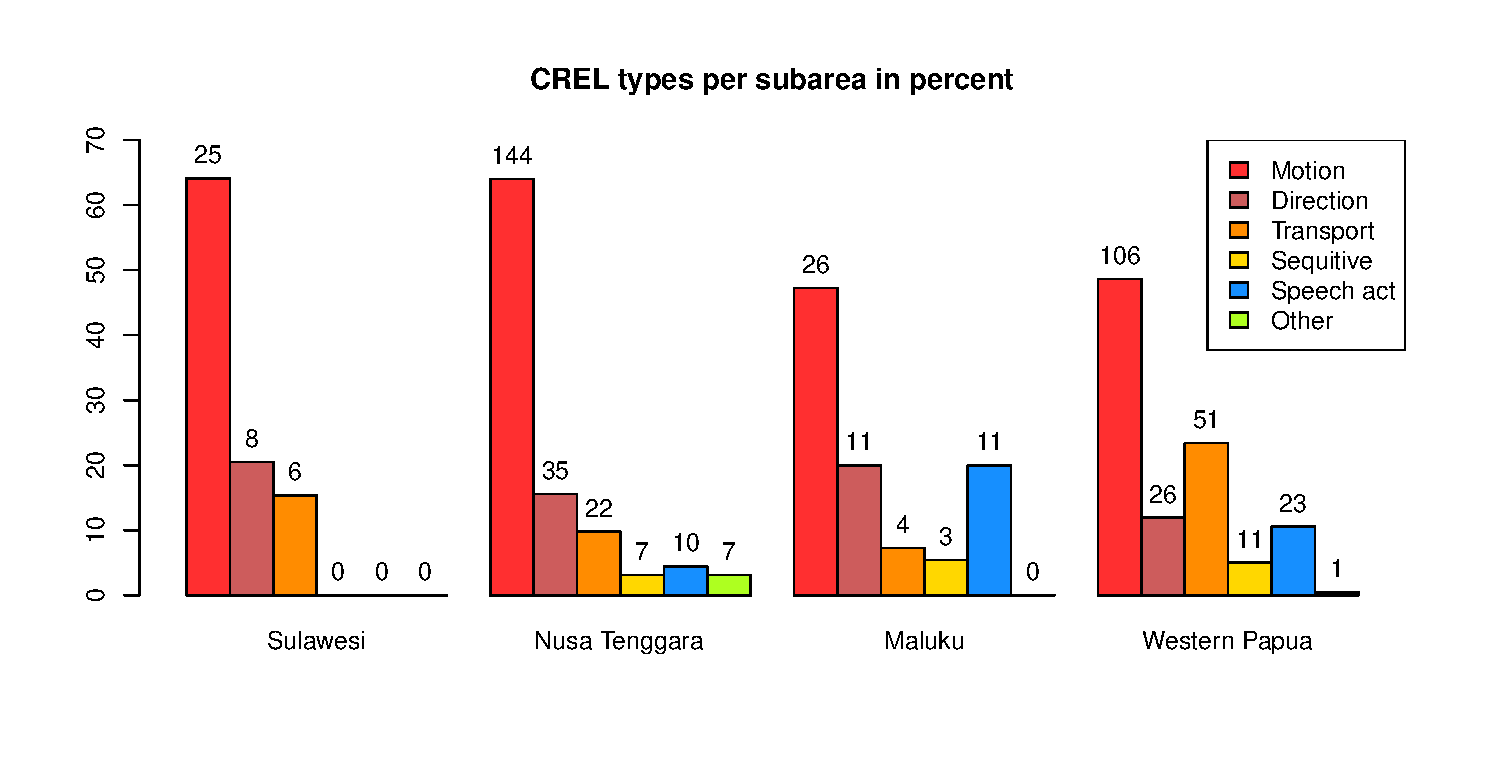
\includegraphics[width=.5\columnwidth]{figures/CREL_Group.eps}
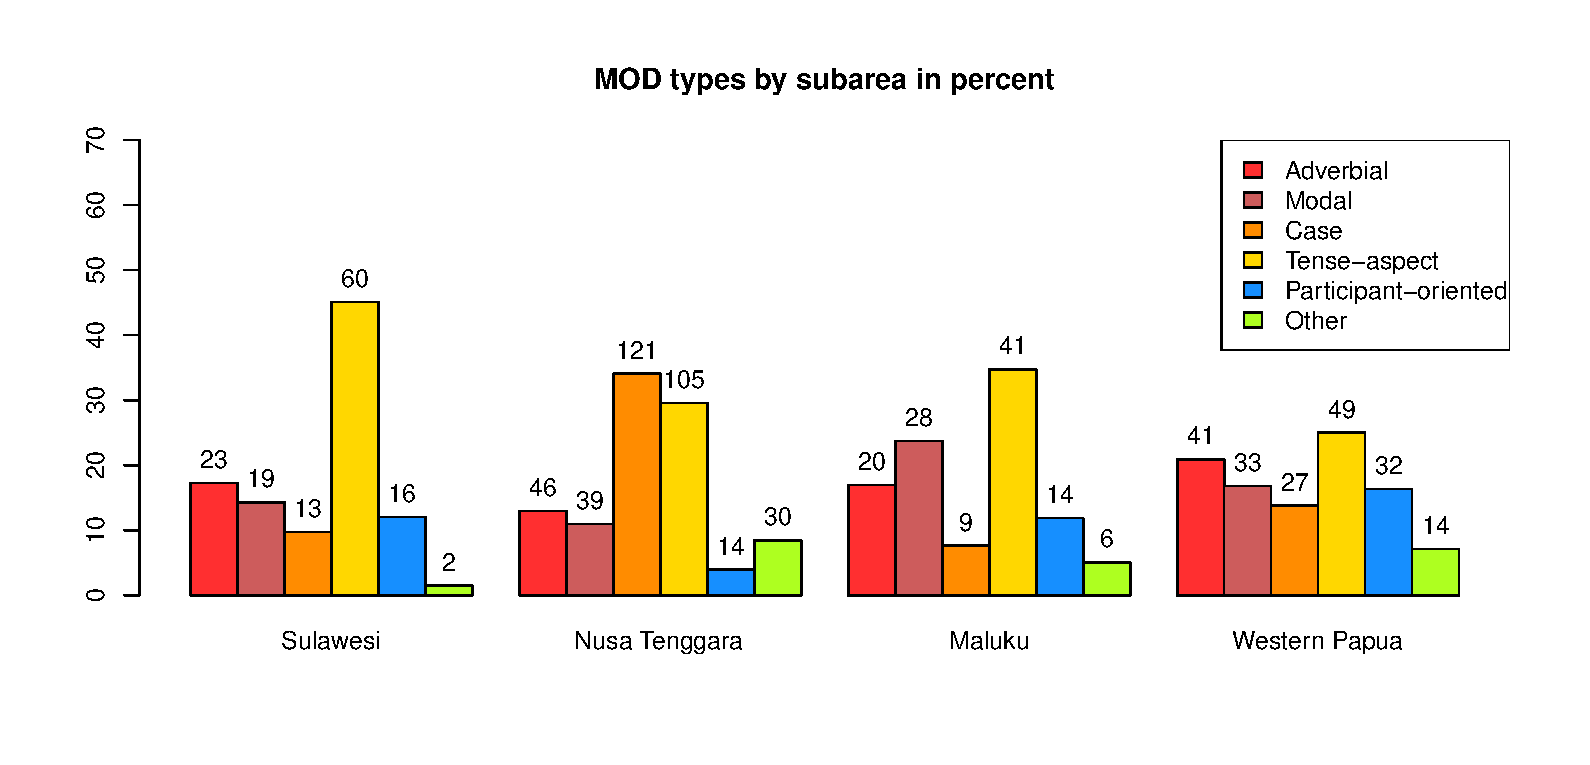
\includegraphics[width=.5\columnwidth]{figures/MOD_Group.eps}
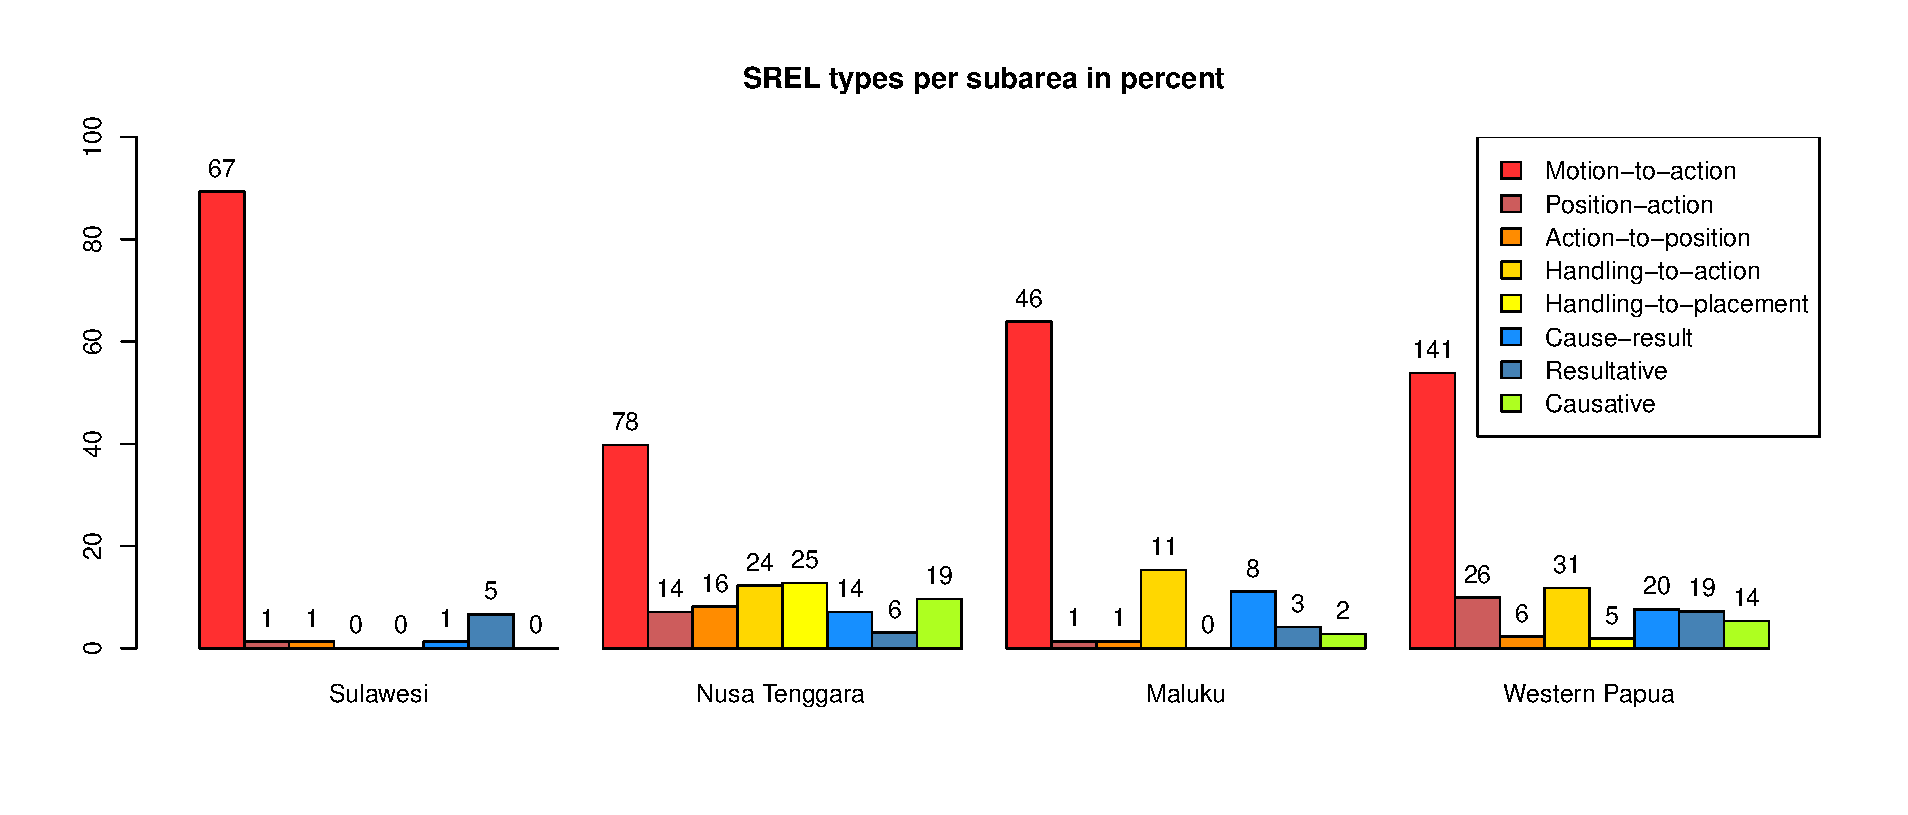
\includegraphics[width=.5\columnwidth]{figures/SREL_Group.eps}
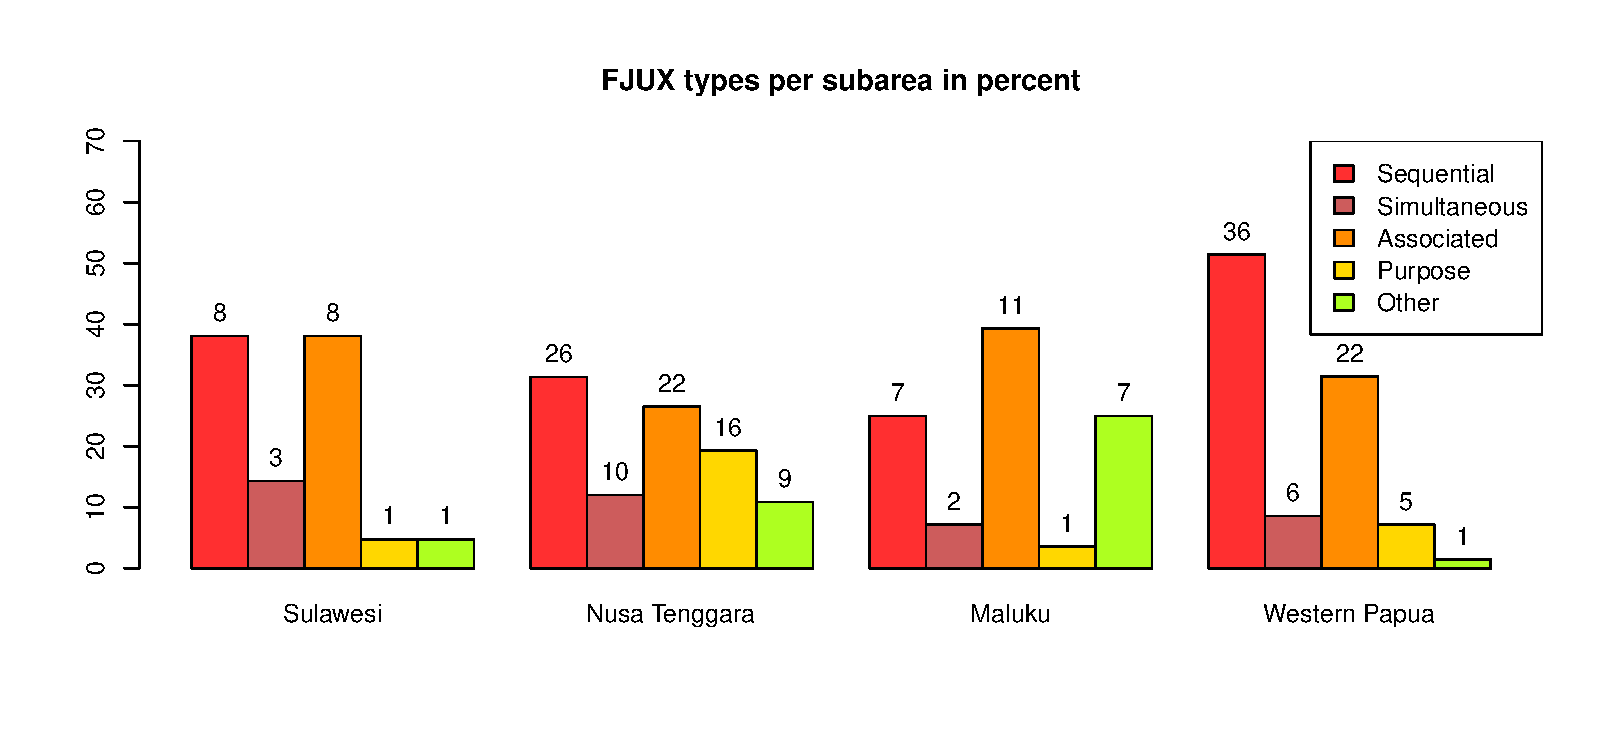
\includegraphics[width=.5\columnwidth]{figures/FJUX_group.eps}
\caption[MVCs per subarea in percent]{MVCs per subarea in percent. This is a composite of Figures \ref{fig:crel-group}, \ref{fig:mod-group}, \ref{fig:srel-group} and \ref{fig:fjux-group} from Chapter \ref{ch:constructions}. CREL = component-relating constructions, SREL = stage-relating constructions, MOD = modifying constructions, FJUX = free juxtaposition constructions. Numbers on top of the bars refer to the number of occurrences.}\label{fig:MVCs_subarea}
\end{minipage}
\end{sidewaysfigure}

In order to further explore the degree of MVC use across the EI languages let us have a look at another indicator. The data from the Figures in \ref{fig:MVCs_subarea} do not tell us how productively the formation of MVCs is integrated into the grammar of a given language. What I want to propose here is an examination of the number of different constructions attested per language. One could wonder whether languages which contribute many examples of MVCs show more attested constructions than languages with only peripherally developed means of MVC formation. Figure §\ref{fig:number_types} below is a calculation of all attested constructions per language as annotated in the EI sample (recall that MOD constructions have been collapsed into functional groups; here, I count all MOD constructions). Let us call this the ``D-score" of the EI languages, indicating the amount of constructional diversity found in each language. The numbers of the D-score are in part predictable from what has been said before. The peaks in the Papuan languages Abui, Makalero, and Maybrat are not surprising as these languages have contributed many examples to the discussion in the previous chapters. Some other languages also contribute high numbers, such as the two corpus languages Waima'a and Wooi, or the Papuan language Tidore from Maluku. Other peaks are more remarkable. The south-eastern Sulawesi languages all contribute more constructions than one might have expected from Figure §\ref{fig:MVCs_subarea} shown above. It is here that the wealth of MOD constructions in these languages becomes visible. With 25 attested constructions, Muna shows the highest number among the Sulawesi languages, clearly contradicting the peripheral status of Sulawesi with regard to MVC use.

\begin{sidewaysfigure}
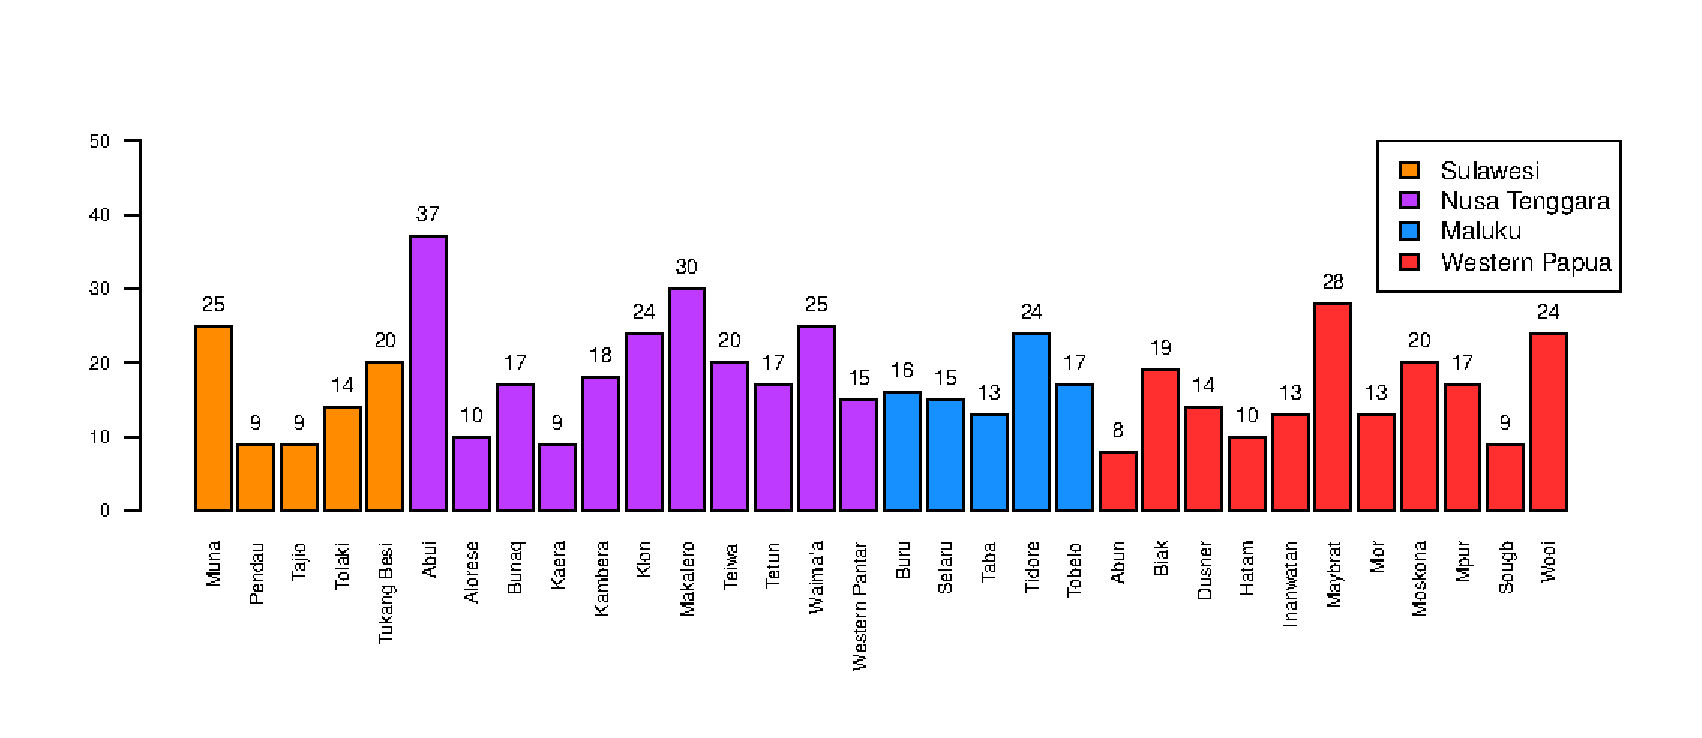
\includegraphics[width=\columnwidth]{figures/MVCs_languages_clean.eps}
\caption[Number of multi-verb constructions per language (``D-score")]{Number of multi-verb constructions per language (``D-score").}\label{fig:number_types}
\end{sidewaysfigure}

However, the calculation from Figure \ref{fig:number_types} would only be representative if we assumed that the numbers were to show the complete inventory of constructions in use in the languages. This is, of course, not the case, since the source data material is limited. Therefore, we need to account for potential undetected constructions. For instance, both in Kaera from the Nusa Tenggara subarea, and in Pendau and Tajio from Sulawesi, a total of nine different constructions is attested. One could draw the conclusion from these numbers that all three languages might have roughly the same degree of MVC use. However, a look at the amount of data points from each language reveals that Kaera only contributed 24 data points, while Tajio contributed 32 data points, and Pendau contributed as many as 51. Therefore it appears more likely that, with 51 data points at hand as in Pendau, the probability of detecting more constructions would be higher than with just 24 instances. Or put differently, the probability of undetected constructions is likely to grow smaller the more data points are added. This assumption holds true, of course, for all languages in the EI sample, which is why the total number of observation matters. The scatterplot in Figure \ref{fig:constructions_tokens} below illustrates the ratio between the number of constructions and the number of data tokens in the EI languages. We can see that, as we move from left to right, the more data enter the game the more constructional types are found on average. Only when the amount of data becomes rather large does the number of detected constructions cease to grow. That is, while the trend is visible for virtually all languages for which published data were used, the two corpus languages, displayed on the far right, strongly suggest that, beyond a certain point, the bulk of constructions is detected and the likelihood of finding new constructions becomes small, no matter how much more data is added.

\begin{sidewaysfigure}
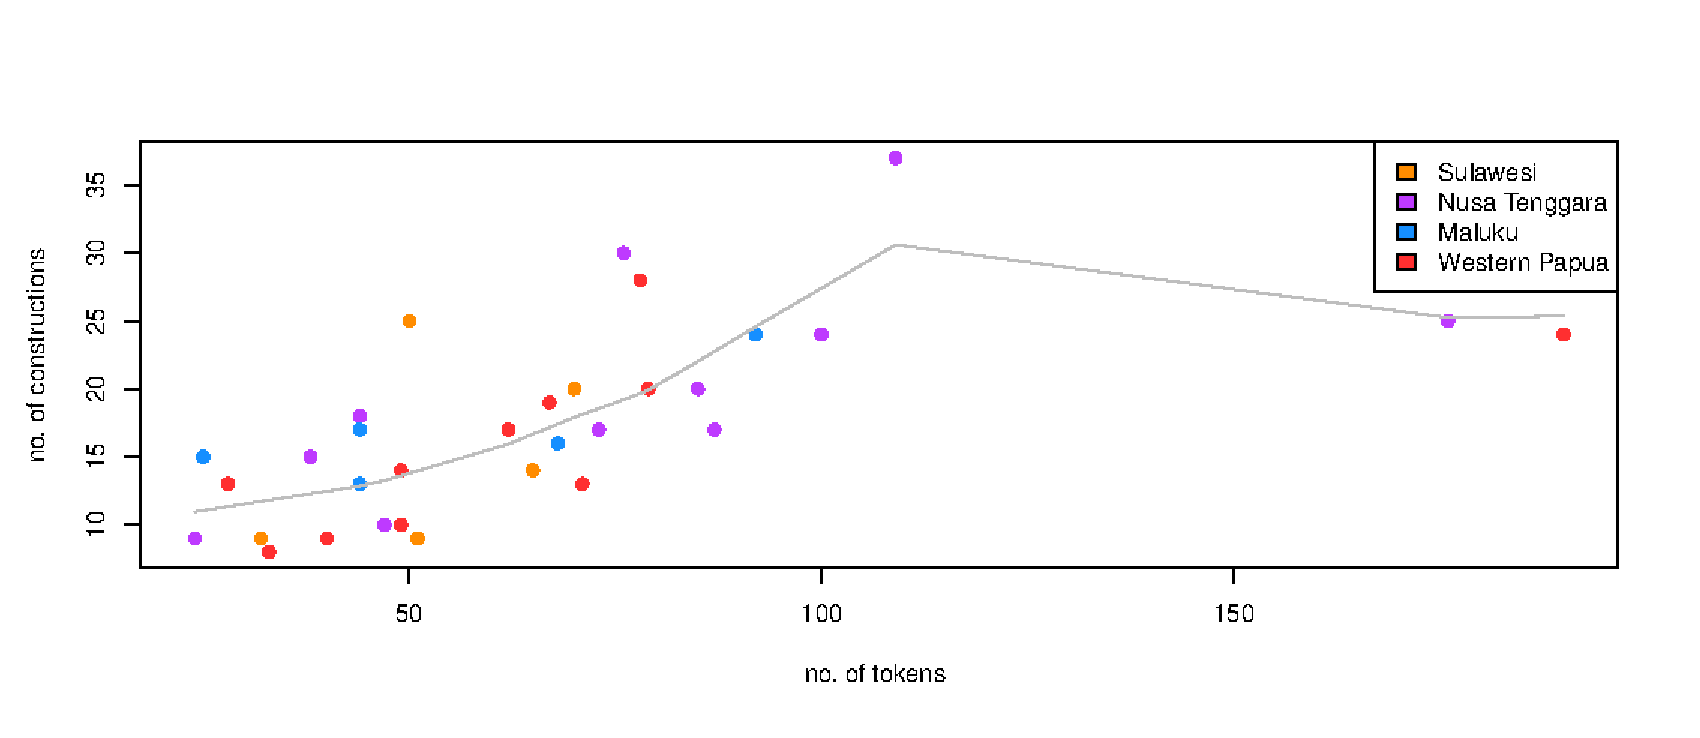
\includegraphics[width=\linewidth]{figures/constructions_tokens_clean.eps}
\caption[Correlation between number of constructions and number of tokens]{Correlation between number of constructions and number of tokens. Each dot represents one language from the EI sample. The dots to the far right belong to Waima'a (violet) and Wooi (red).}\label{fig:constructions_tokens}
\end{sidewaysfigure}

This observation leaves us with two potential factors that would need to be accounted for when we talk about MVC use. First, we have the number of attested constructions per language (n$_c$), i.e., a rough indicator of constructional diversity. And second, we have the number of observations or data tokens per language (n$_t$), i.e., a very rough measure of frequency of constructional use. Table \ref{table:diversity_language} below returns the numbers of each factor. A simple way to relate these would be to divide the number of constructions by the number of tokens. The results are also displayed in Table \ref{table:diversity_language}. This index provides the frequency of attested constructions per number of data tokens. For instance, Muna has an index of 0.5, meaning that we end up with one detected construction for every two data tokens. This index, however, would only work well if the chance to detect new constructions would be the same across all languages. But this is clearly not the case. Selaru is a good test case in this regard. Selaru only contributed 25 data points to the sample. The reason for such a low number is that Selaru predominantly uses a set of linkers, \textit{ti} and \textit{ma} (probably derived from motion verbs), to link verbs together. So, despite the fact that a whole grammar was searched for multi-verb constructions, very few were found. Thus, in this case we probably would not get significantly more constructions if we were to examine another source of Selaru data. Table \ref{table:diversity_language} in fact shows a higher value for Selaru (0.6) than for, say, Abui (0.34), although Abui has the highest score of attested constructions (37). Note also that the corpus languages, Waima'a and Wooi, return extremely low numbers owing to the effect of a large corpus size outlined above. Such a frequency index clearly does not return reliable values. For the time being, I therefore stick to the number of constructions attested for each language, the D-score. In §\ref{sec:profile_use}, I will take up these numbers in order to present different profiles of MVC use throughout the EI area.

\begin{table}
\begin{footnotesize}
\begin{tabular}{l r r r}
  \lsptoprule
  \\
& n$_c$ & n$_t$ & $\frac{n_c}{n_t}$ \\ 
\\
  \hline
Muna	& 25 &	50 &	0.5	 \\
Pendau	& 9 &		51 &	0.18 \\
Tajio	& 9 &		32 &	0.18 \\ 
Tolaki	& 14 &	65 &	0.22 \\
Tukang Besi &	20 &	70 &	0.29 \\ \hline
Abui	& 37 &	109 &	0.34 \\
Alorese	& 10 &	47 &	0.21 \\
Bunaq	& 17 &	87 &	0.2	 \\
Kaera	& 9 &		24 &	0.38 \\
Kambera	& 18 &	44 &	0.41 \\
Klon	& 24 &	100 &	0.24 \\
Makalero &	30 &	76 &	0.39 \\
Teiwa	& 20 &	85 &	0.24 \\
Tetun	& 17 &	73 &	0.23 \\
Waima'a	& 25 &	176 &	0.14 \\
Western Pantar	& 15 &	38 &	0.39 \\ \hline
Buru	& 16 &	68 &	0.24 \\
Selaru	& 15 &	25 &	0.6	 \\
Taba	& 13 &	44 &	0.3	 \\
Tidore	& 24 &	92 &	0.26 \\
Tobelo	& 17 &	44 &	0.39 \\ \hline
Abun	& 8 &	33 &	0.24 \\
Biak	& 19 &	67 &	0.28 \\
Dusner	& 14 &	49 &	0.29 \\
Hatam	& 10 &	49 &	0.2	 \\
Inanwatan	& 13 &	28 &	0.46 \\
Maybrat	& 28 &	78 &	0.36 \\
Mor	& 13 &	71 &	0.18	 \\
Moskona	& 20 &	79 &	0.25 \\
Mpur	& 17 &	62 &	0.27 \\
Sougb	& 9 &	40 &	0.23 \\
Wooi	& 24 &	190 &	0.13 \\
\lspbottomrule
\end{tabular}
\end{footnotesize}
\caption[Diversity of multi-verb constructions per language]{Diversity of multi-verb constructions per language. n$_c$ = number of constructions, n$_t$ = number of tokens, $\frac{n_c}{n_t}$ = frequency index of constructions per number of tokens.}
\label{table:diversity_language}
\end{table}

In order to arrive at statistically relevant results one would need to normalise the number of tokens examined for each language. For instance, if for each language the same number of IPs defined on the basis of comparable boundary signals were explored in terms of n$_c$ and n$_t$, more accurate values could be obtained. This was for practical reasons beyond the scope of this book. What I want to propose here is that the D-score, i.e., the number of constructions found, can give at least a rough idea of the degree to which multi-verb constructions pervade the grammatical system of individual languages in Eastern Indonesia.\footnote{An anonymous reviewer pointed out that diversity of multi-verb constructions is not necessarily related to frequency of use. This is certainly true. What I intended to stress by comparing the number of constructions with the number of tokens is that the ratio between them is quite different across the individual languages, and that this may be meaningful. Recall that the sample does not only consist of data points deliberately provided in the source publications as examples of verb serialisation, but also of examples collected from sections and chapters totally unrelated to the discussion of verb serialisation. Languages with many data points but few attested constructions therefore appear to have a smaller repertoire of multi-verb constructions at their disposal, although this clearly needs further checking.}

\section{Hierarchy in MVCs} \label{sec:hierarchy}

Hierarchy in linguistic structure is typically accompanied by grammatical marking. Subordinate clauses, for instance, are flagged with non-finite or reduced verb morphology in many languages, or with grammatical formatives of some sort. The same applies to structures in which hierarchies could be expected, but where none are intended. Think of structures where conjunctive elements explicitly coordinate constituents that are on the same rank. Such devices are only sporadically encountered in Eastern Indonesia. Many EI languages lack an elaborate set of junctors, and Indonesian loan junctors are sometimes used as a result of increased diglossia and exposure to regional Malay varieties. Native formatives that flag co- or subordination are rare in many EI languages. When there are morphological means to flag certain types of clause linkage, these overt constructions often replace MVCs. For instance, Kambera has developed a proclitic \textit{pa=} denoting that the flagged constituent is controlled by a matrix clause (see \citealt[338ff.]{klamer1998grammar}). The proclitic is found, among others, in clause combinations that appear to function just like motion-to-action MVCs (but convey a purposive reading, or so it seems). Or, to mention another example, Abun has a simultaneous-events construction flagged by the clitic \textit{=i}. The clitic is attached to clause-final position when two events happen at the same time \citep{berry1999}. Those cases have not been counted as simultaneous FJUX constructions, although functionally they bear some resemblance.

As MVCs are basically verb strings without grammatical marking, it comes as no suprise that very little has been written on hierarchies in MVCs, or in SVCs, for that matter. We have already seen in §\ref{sec:literature-mvcs} that \citet{enfield2008verbs} provides an insightful analysis of MVCs in Lao, explicitly stating that many complex verb strings in Lao may be dissected into mostly binary V$_1$-V$_2$ combinations. Reconsider example (\ref{lao1}) (here repeated as (\ref{lao_2})) from Lao with six verbs in sequence.

\ea \label{lao_2}
\langinfo{Lao}{Tai-Kadai}{\citealt[83]{enfield2008verbs}}\\
\gll caw$^4$ lòòng$^2$ mèè$^4$ qaw$^3$ paj$^3$ hêt$^1$ kin$^3$ beng$^1$ \\
2\textsc{sg} try.out \textsc{ptl} take go make eat look \\
\glft `You go ahead and take (them) and try cooking (them)!'\\ 
\z

This utterance, as Enfield remarks, constitutes ``a single prosodically integrated unit", and \begin{quote}is no mere `string of verbs'. Such sequences in Lao can be analysed in terms of nested (usually binary) relationships. In [the above] example [...], a left-headed complement-taking adverbial \textit{lòòng$^2$} `try out' combines with a right-marking adverbial \textit{beng$^1$} `look' in bracketing a complex verb phrase consisting of a `disposal' construction expressing focus on manipulation of the object (with the combination \textit{qaw$^3$-hêt$^1$} `take (and) do/make'), incorporating \textit{paj$^3$} `go' as an inner directional particle, in a purposive clause chain with \textit{kin$^3$} `eat'. The surface string of six contiguous verbs [...] is highly structured, yet there is little if any surface indication of such structure in the language. \citep[83]{enfield2008verbs}\end{quote}

The verb combinations from the Lao example are strikingly similar to what we have seen in Chapter \ref{ch:constructions}, and the EI constructions may be stacked, or nested, in much the same way as in the Lao string. Example (\ref{KYO001a}) from Klon is certainly an extreme case of stacked MVCs in EI, but serves to illustrate how deep such recursive MVCs may extend. 

\ea \label{KYO001a}
\langinfo{Klon}{Papuan, TAP}{\citealt[140]{baird2008grammar}}\\
\gll pi brai brai lam agai nmei mi hos koh di, pi pa u-eel\\
\textsc{1}\textsc{nsg}.\textsc{in}.\textsc{act} slow slow walk go place be.at put finish first \textsc{1}\textsc{nsg}.\textsc{in}.\textsc{act} \textsc{1}\textsc{nsg}.\textsc{in}.\textsc{hor} \textsc{vi}-stop\\
\glft `We walked slowly, putting (them) in the place, then we rested, [...]'\\ 
\z

The MVC in (\ref{KYO001a}) comprises six verbs in sequence, up to \textit{koh} `finish' (disregarding the repetition of \textit{brai}). The verbs appear to fall into two groups: the first three verbs denote a motion event, slowly walking away from some discourse origo. Two motion verbs, \textit{lam} `walk' and \textit{agai} `go', are merged in order to form a \textsc{motion complex} MVC. The result of this merger is, on the next higher level, modified by \textit{brai} `slow'. I analysed such modifying relations as adverbial MOD MVCs in §\ref{sec:modification}. The verb triplet on the right hand side is internally structured in similar ways. Here it is two modifier verbs that attach at different levels. I assume that modification of \textit{hos} `put' by the locative verb \textit{mi} `be at' constitutes the inner MVC, and that the resulting case-marking MOD MVC is again modified by the aspectual verb \textit{koh}.\footnote{There are particular difficulties associated with interpreting the exact scope of modifier verbs, as has already become clear from the discussion in §\ref{sec:clauselevelmodification} on clause-level modification. In this case, an alternative analysis could treat the left-peripheral modifier \textit{brai} and the right-peripheral modifier \textit{koh} as having scope over the whole construction, resulting in a reading like `slowly, we walked away (and) put (them) in place (until) done'. I see no reason why this reading should not, in principle, be available as well, although a repetition of \textit{brai} seems more intimately connected to a process like walking rather than to an accomplishment like putting. Yet I assume that the preferred interpretation of such modifiers, especially in complex hard-to-parse structures like this one, is partial scope over neighbouring discernable event units.} At the topmost level we can recognise the by now familiar combination of a motion stage followed by an action stage, that is, the whole string is likely to be interpreted as a motion-to-action MVC. Figure \ref{figure:eventschema_KYO001a} illustrates the internal structure of the whole sequence by applying the insights from Chapter \ref{ch:sem}. The event arguments, percolating upwards as the verbs combine to form event schemas on higher levels, spring from the dynamic verbs \textit{lam}, \textit{agai}, and \textit{hos}. The former two merge their event arguments, filling the event argument of the motion stage at the topmost level of the tree. The event argument from \textit{hos} percolates upwards and becomes the event argument of the action stage. The modifier verbs instead contribute empty event arguments that adapt to those of the matrix verbs.

\begin{sidewaysfigure}

\jtree[xunit=10em,yunit=2em]
\defbranch<shortleft>(1)(2.2)
\defbranch<shortright>(1)(-2.2)

\defstuff[a]{\multiline
{CLE -- motion-to-action (staged)}\cr
{\begin{scriptsize} [[ \textbf{do'} (we, \textbf{move'} (we, \textsc{path=\rnode{A3}{go}}, \textbf{walk'} (e$_{1=2}$, we))) \&  \textsc{slow} (e$_{1=2}$, we)] \& \end{scriptsize}}\cr
{\begin{scriptsize} [ \textsc{become} \textbf{do'} (we, \textbf{move'} (we, \textsc{path}, \textbf{put'} (e$_3$, we, (them)))) \&  \textsc{locative} (e$_3$, we) \& \textsc{finish} (e$_3$, we) ]]\end{scriptsize}}
\endmultiline}

\defstuff[b]{\multiline
{PLE -- adverbial modifying}\cr
{\begin{scriptsize}[ \textbf{do'} (we, \textbf{move'} (we, \textsc{path=go}, \textbf{walk'} (e$_{1=2}$, we))) \& \end{scriptsize}}\cr
{\begin{scriptsize} \textsc{\rnode{S4}{slow}} (\rnode{T4}{e$_{1=2}$}, we) ]\end{scriptsize}}
\endmultiline}

\defstuff[c]{\multiline
{PLE -- aspectual modifying}\cr
{\begin{scriptsize} [ \textsc{become} \textbf{do'} (we, \textbf{move'} (we, \textsc{path}, \textbf{put'} (e$_3$, we, (them)))) \& \end{scriptsize}}\cr
{\begin{scriptsize} \textsc{locative} (e$_3$, we) \& \textsc{\rnode{F4}{finish}} (\rnode{P7}{e$_3$}, we) ]\end{scriptsize}}
\endmultiline}

\defstuff[d]{\multiline
{PLE -- case modifying}\cr
{\begin{scriptsize} [ \textsc{become} \textbf{do'} (we, \textbf{move'} (we, \textsc{path}, \textbf{\rnode{P3}{put'}} (\rnode{P6}{e$_3$}, we, (them)))) \& \end{scriptsize}}\cr
{\begin{scriptsize} \textsc{\rnode{F2}{locative}} (\rnode{P5}{e$_3$}, we) ]\end{scriptsize}}
\endmultiline}

\defstuff[e]{\multiline
{PLE -- motion complex}\cr
{\begin{scriptsize}\textbf{do'} (we, \textbf{move'} (we, \textsc{path=\rnode{A3}{go}}, \textbf{\rnode{D4}{walk'}} (e$_{\rnode{C3}{1}=\rnode{B3}{2}}$, we)))\end{scriptsize}}
\endmultiline}

\! = {\stuff[a]}
<left>{\stuff[b]}!a ^<right>{\stuff[c]}
<left>[xunit=0.5em]{\stuff[d]}!b ^<right>[linestyle=dotted]{PLE}
<vert>{LLE}
<vert>{\textit{koh}}
{\begin{scriptsize} \textsc{\rnode{F3}{finish}} (e''', we)\end{scriptsize}}.

\!a = <left>[linestyle=dotted]{PLE}!c ^<right>[xunit=0.5em]{\stuff[e]}
<shortleft>{LLE}!d ^<shortright>{LLE}
<vert>[scaleby=1.6]{\textit{agai}}
{\begin{scriptsize} \textbf{do'} (we, \textbf{move'} (we, \textsc{path=\rnode{A2}{go}}, \textbf{go'} (\rnode{B2}{e$_2$}, we)))\end{scriptsize}}.

\!b = <shortleft>{LLE}!e ^<shortright>{LLE}
<vert>[scaleby=1.6]{\textit{hos}}
{\begin{scriptsize} \textsc{become} \textbf{do'} (we, \textbf{move'} (we, \textsc{path}, \textbf{\rnode{P2}{put'}} (\rnode{P4}{e$_3$}, we, (them))))\end{scriptsize}}.

\!c = <vert>{LLE}
<vert>{\textit{brai}}
{\begin{scriptsize} \textsc{\rnode{S3}{slow}} (e', we)\end{scriptsize}}.

\!d = <vert>{\textit{lam}}
{\begin{scriptsize} \textbf{do'} (we, \textbf{move'} (we, \textsc{path}, \textbf{\rnode{D1}{walk'}} (\rnode{B1}{e$_1$}, we)))\end{scriptsize}}.

\!e = <vert>{\textit{mi}}
{\begin{scriptsize} \textsc{\rnode{F1}{locative}} (e'', we)\end{scriptsize}}.

\psset{linestyle=dotted,angleA=45,angleB=-90,arrows=->}
\nccurve{A2}{A3} %von TRANS hoch zu TRANS-motion complex
\nccurve{B2}{B3} % von e2-go zu e2-motion complex
\nccurve{P2}{P3} % von put zu put-case mod
\nccurve{C3}{T4} %von motion complex = hoch zu e-slow
\nccurve{P4}{P5} % von e3-put zu e3-put-case mod
\nccurve{P4}{P6} % von e3-put zu e3-put-case mod
\nccurve{P6}{P7} % von e3-put zu e3-put-asp mod
\psset{linestyle=dotted,angleA=70,angleB=-45,arrows=->}
\nccurve{F3}{F4} %von finish hoch zu finish-aspec
\psset{linestyle=dotted,angleA=100,angleB=-100,arrows=->}
\nccurve{B1}{C3} %von e1-walk zu e1- motion complex
\nccurve{D1}{D4} %von walk hoch zu walk-motion complex
\nccurve{S3}{S4} %von slow zu adv-slow
\nccurve{F1}{F2} %von locative hoch zu case-locative
\endjtree

\caption[Event schema illustration of example (\ref{KYO001a})]{Illustration of the composite event schema of example (\ref{KYO001a}). LLE -- \textsc{lexeme-level event}, PLE -- \textsc{predicate-level event}, CLE -- \textsc{clause-level event}.}
\label{figure:eventschema_KYO001a}
\end{sidewaysfigure}

The challenge with such verbal interactions is to decide whether we are looking at structural dependencies as found, for instance, in many languages of Europe and Central Asia, or whether we are in fact dealing with paratactic formations, as \citep[151]{levinson2013recursion} remarks. Discussing recursion from a pragmatic perspective, Levinson points out that center-embedding, that is, a subordinate construction embedded on both sides into a matrix structure (ABBA), may be grammatically licit, but at a certain depth runs into severe parsing problems, so that center-embedding in oral language is practically capped at two levels deep (three in written language; \citealt[154]{levinson2013recursion}). While recursion by center-embedding is unambiguous and can be detected with ease, this is not the case for edge-recursion where dependencies are not structurally visible, as the embedded construction is only flanked on one side. It appears that recursion in EI MVCs is almost always edge-recursion, as cases of center-embedding are lacking. Take example (\ref{KYO001a}) again. Embedding takes place two levels deep. Starting from the motion-to-action matrix level, the motion stage branches off to the left, while the action stage branches off to the right. The resultant modifying MVCs then both exhibit edge-recursion directed towards the inner edge. Note, however, that we do not get a structure like ABA, say, (\textit{brai}(\textit{lam})\textit{agai}), so any lower-ranked MVC in example (\ref{KYO001a}) is a case of edge-recursion. The only cases of cross-serial dependencies in EI MVCs are found in motion complex MVCs from languages with AOV order which are modified by a locative verb marking the goal of the motion event. Example (\ref{Kaera_13}) from Kaera is such a rare case. The two motion verbs flank the modifier verb in center position, but note that the modifying MVC is the matrix-level construction, as it modifies the whole motion complex, and not just one of the motion verbs. So, we are not in fact dealing with center-embedding here, but with discontinuous edge-recursion.

\ea \label{Kaera_13}
\langinfo{Kaera}{Papuan, TAP}{\citealt[138]{klamer2014kaera}}\\
\gll wer bir~bir ming, gang ekeng abang wang gi \\
sun \textsc{rdp}~run be 3\textsc{sg} climb.up village be go \\
\glft `At midday, she went up to the village.'\\ 
\z

Constraints on cross-serial dependencies in MVCs are in all likelihood due to obvious parsing problems. The longer a string of verbs gets, the more readings are possible. The lack of structural flagging is compensated by compiling such strings in paratactic patterns. Ease of parsing, however, does not preclude edge-recursion, and in compliance with the semantic approach outlined in chapter \ref{ch:sem}, we can identify a wealth of mostly binary verb--verb relationships within MVCs. Remarkably, internal structure of this sort is not observed in all constructional MVC families. Component-relating constructions have not been found with embedded MVC constructions, indicating their coherent one-staged semantic construal.

The fact that MVCs in EI can be stacked begs the question whether all EI languages allow stacking, and if so, to which extent? This question takes us back to the issue of MVC use and diversity in the EI region. As a hypothesis one may assume that languages with heavy use of MVCs show more MVC embedding than languages with only peripheral use of MVCs. As every construction in the EI sample has been annotated according to its hierarchical position, we can calculate the number of stacked MVCs by counting the number of matrix-level MVCs. Figure \ref{fig:stacked} illustrates the number of stacked MVCs observed for each language.

\begin{sidewaysfigure}
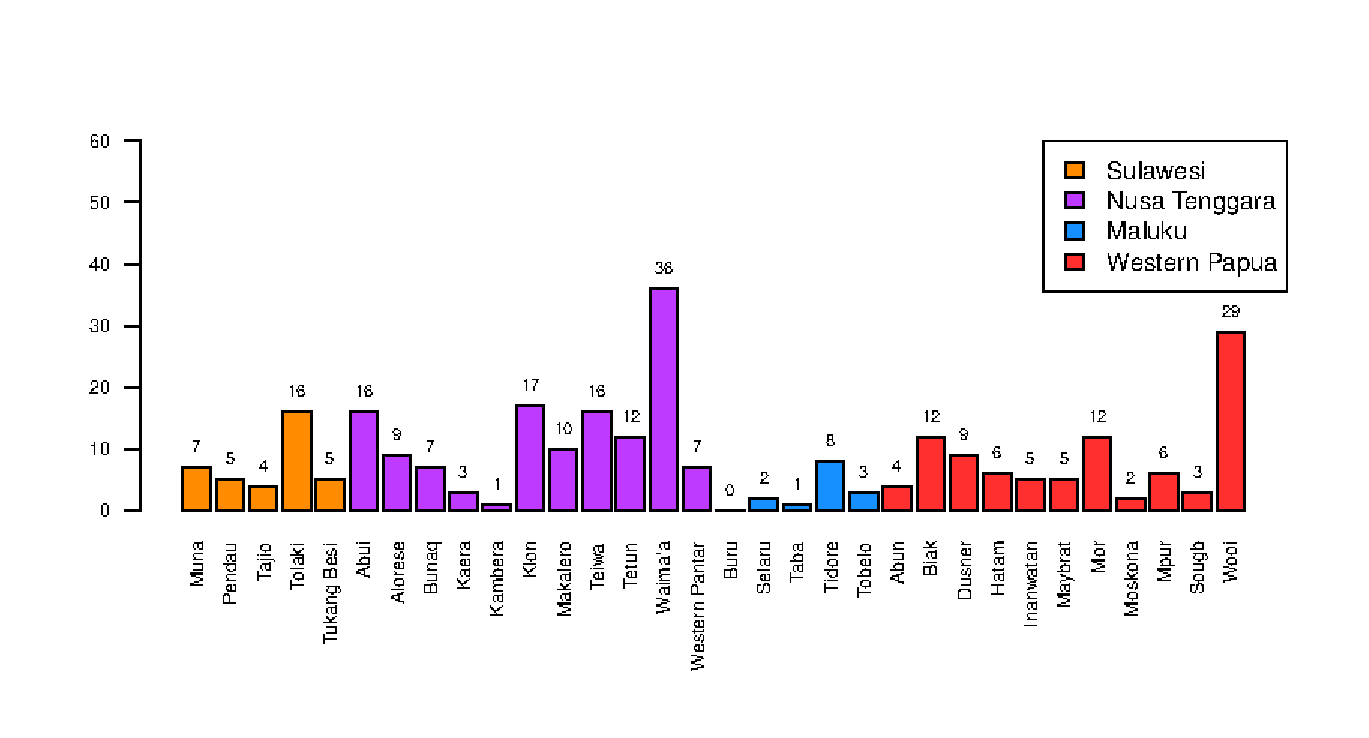
\includegraphics[width=\textwidth]{figures/number_stackedMVC_clean.eps}
\caption[Number of stacked MVCs per language]{Number of stacked MVCs per language.}\label{fig:stacked}
\end{sidewaysfigure}

Two observations arise from these numbers. First and counterintuitively, the amount of stacking does not necessarily correlate with the D-score from §\ref{sec:distribution}. While the Sulawesi group shows intermediate numbers of stacking, the numbers from the Maluku group are lower than expected. If we specifically compare the northern Sulawesi group Pendau and Tajio with the group of Austronesian Maluku languages, Buru, Selaru and Taba, this distribution contradicts the trend from the D-score illustrated in Figure \ref{fig:number_types}. And second, the two corpus languages, Waima'a and Wooi, fare especially well although they only show average D-score values. If the two languages with most data points score best, the distribution is obviously unbalanced. Therefore we need to take into account the total number of MVC observations per language (n$_t$). As in §\ref{sec:distribution}, I computed a frequency index by dividing the number of stacked MVCs by the total number of MVC observations. The results are illustrated in Figure \ref{fig:complexity} below. As we are not dealing with a count of different types, as with the number of construction types in §\ref{sec:distribution}, but with the sum of observations of one particular value (=stacked), this index arguably is a slightly better predictor of MVC complexity than the frequency index from Table \ref{table:diversity_language}. Therefore, I used this index instead of the mere number of stacked MVCs per language, as illustrated in Figure \ref{fig:stacked}. I call it the C-score (complexity score), analogous to the D-score from the last section.

We can gather from the C-score values in Figure \ref{fig:complexity} that the peaks of the two corpus languages are levelled out, but the same cannot be said for the values of the Sulawesi languages. Thus, in terms of internal MVC complexity, we can state that both the languages from Nusa Tenggara (with the exception of the western outlier Kambera) and from Western Papua show the highest numbers of stacked MVCs in relation to the size of the data points considered. The Sulawesi languages, including the northern languages, also show rather high numbers of stacked MVCs. Finally and surprisingly, the Maluku languages lag behind in the use of complex MVCs (Selaru has gained a little, but this, again, is probably a chance effect due to the low number of observations). 

\begin{sidewaysfigure}
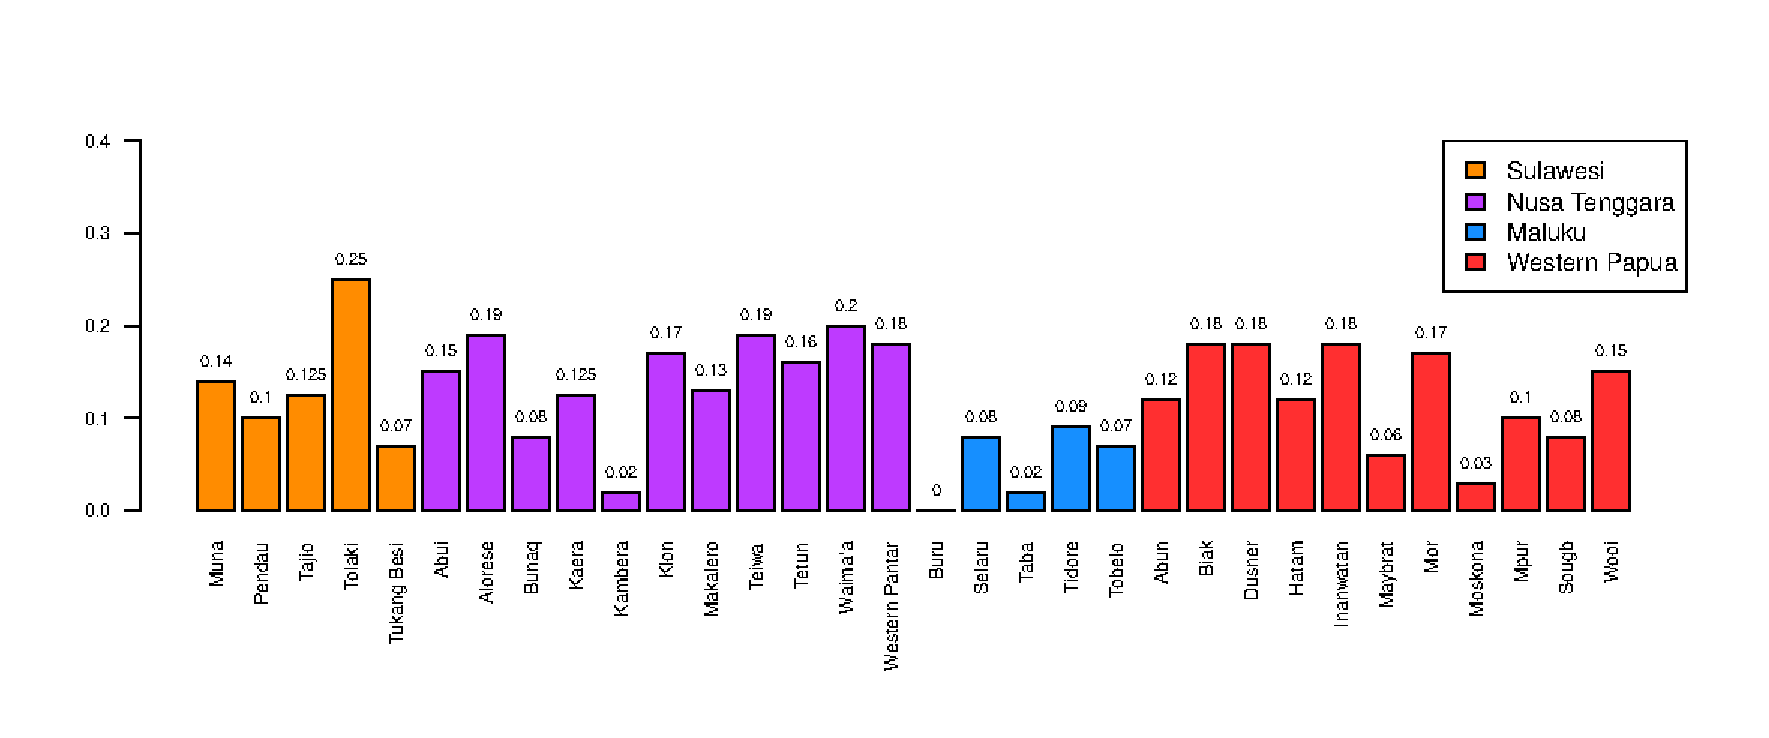
\includegraphics[width=\textwidth]{figures/index_MVCcomplexity_clean.eps}
\caption[Index of MVC complexity per language]{Index of MVC complexity per language (C-score). Explanation in the prose.}\label{fig:complexity}
\end{sidewaysfigure}

In the following section, I will combine the findings from this section and the previous one, and propose a tentative classification of the EI languages according to different profiles of MVC use.

\section{Linguistic profiles of MVC use} \label{sec:profile_use}

We have seen from the last two sections that the D-score (the number of constructions attested) and the C-score (derived from the frequency of complex MVCs relative to the number of observations available) both relate to MVC use in a given language. However, both values show opposing trends for some languages, and thus do not fit well in all cases. On the basis of the limited number of observations available from the EI sample there seems to be no simple \textit{ad hoc} solution that would resolve both factors into a single typology of languages, ranging from languages with little MVC use to languages with high usage. Let us therefore have another look at the C-score. The languages that scored highest in terms of constructional diversity (Abui, Makalero, Muna, and Maybrat) all have average C-values (at best; Maybrat in fact has a very low C-score). Some  languages, on the other hand, that have low D-values fare surprisingly well. This is for example the case with Mor from Western Papua, Alorese and Kaera from Nusa Tenggara, or Pendau and Tajio from Sulawesi. A closer inspection of these languages reveals that it is predominantly cases of motion-to-action MVCs with embedded motion CRELs in the motion slot (motion complex MVCs or transport MVCs) that cause higher numbers of stacked MVCs. Thus, most languages with high C-scores make good use of these constructions, and allow stacking in motion slots of motion-to-action. Given that both motion-to-action and motion complex MVCs are among the most frequent constructions found in the sample, the C-score is slightly skewed towards combinations of motion MVCs.

From what has been said, it seems reasonable to base a typology of MVC use on the D-score rather than on the C-score, and preference is therefore given to the D-score values. Table \ref{table:profile_MVCuse} below outlines a typology of MVC use, and classifies the languages on the basis of their D-score values. I distinguish between four profiles in the EI region: languages with little use of MVCs (rank I), languages with moderate use (rank II), and languages with extensive use (rank III). To these we may add another language profile: languages that do not make use of MVCs altogether (rank 0). Rank 0 languages do not show up in the EI sample because all sample languages were checked for MVC use beforehand, and languages without signs of MVC use had been excluded. The threshold values to define the profiles are derived from the D-score and are largely chosen at arbitrary points. In order to be able to include the C-score results, I computed the C-score mean, which is 0.12, and compared it to the C-score values of the languages. Languages that strongly deviate from this mean are allowed to move up or down one rank. To this end, I computed the standard deviation from the C-score mean ($\pm 0.06$) and defined it as the threshold beyond which a given language would move up or down one rank ($0.12 \pm 0.06$). Any language with a C-score less than 0.06 would be ranked lower, and any language with a C-score greater than 0.18 would be ranked higher. So, for instance, as the C-score of Kambera is only 0.02 the language is ranked down from the moderate use profile to the little use profile. Changes in ranking are displayed by the symbols $\uparrow$ and $\downarrow$, respectively. Note that in the case of Taba I made one exception to this, not allowing a rank I language to move downwards to rank 0. This is because a language that does obviously use MVCs of quite different sorts can hardly be classified as having no MVC use at all. Table \ref{table:profile_MVCuse} illustrates the different profiles, and sorts the EI languages according to the procedure just discussed.

\begin{table}
\begin{footnotesize}
\begin{tabular}{r l l p{5cm} }
\lsptoprule
Rank & Profile & D-score threshold & Languages \\
 \\ 
\hline
 Rank III & extensive MVC use & $D > 24 $ & Muna, Abui, Makalero, Teiwa$\uparrow$, Waima'a, Maybrat \\ 
\hline 
Rank II & moderate MVC use & $  15 \leq D \geq 24 $ & Tolaki$\uparrow$, Tukang Besi, Alorese$\uparrow$, Bunaq, Klon, Tetun, Western Pantar, Selaru, Tidore, Tobelo, Biak, Mpur, Wooi \\
\hline
Rank I & little MVC use & $ 5 \leq D \geq 14 $  & Pendau, Tajio, Kaera, Kambera$\downarrow$, Buru$\downarrow$, Taba($\downarrow$), Abun, Dusner, Hatam, Inanwatan, Mor, Moskona$\downarrow$, Sougb \\
\hline 
Rank 0 & (almost) no MVC use & $ D < 5 $ & \textit{none in EI sample} \\    
\lspbottomrule 
\end{tabular}
\end{footnotesize}
\caption[Linguistic profiles of MVC use]{Linguistic profiles of MVC use. Languages with a C-score below or above standard deviation ($D < 0.06$ or $D > 0.18$) are ranked lower or higher. Reranked languages are marked with $\downarrow$ and $\uparrow$, respectively. Taba was chosen to be left in rank I and not moved down (indicated by the brackets).}
\label{table:profile_MVCuse} 
\end{table}

A comparison of the results from Table \ref{table:profile_MVCuse} with the D-score values shows that all four languages that scored highest reappear in the `extensive use' profile: Muna, Abui, Makalero, and Maybrat. One further language from Nusa Tenggara, Teiwa, has been promoted upwards due to high C-scores. Most other EI languages are classified as showing moderate MVC use (n=15), while another sizeable group are ranked as `little MVC use' (n=13). As might be predicted, among these rank I languages, we predominantly find languages from the periphery of the EI region: the two northern Sulawesi languages Pendau and Tajio belong to this group, as well as the western outlier Kambera from the Nusa Tenggara subarea, and also the Austronesian languages Dusner and Mor located in the southern part of Cenderawasih Bay (Western Papua group). 

\begin{sidewaysfigure}
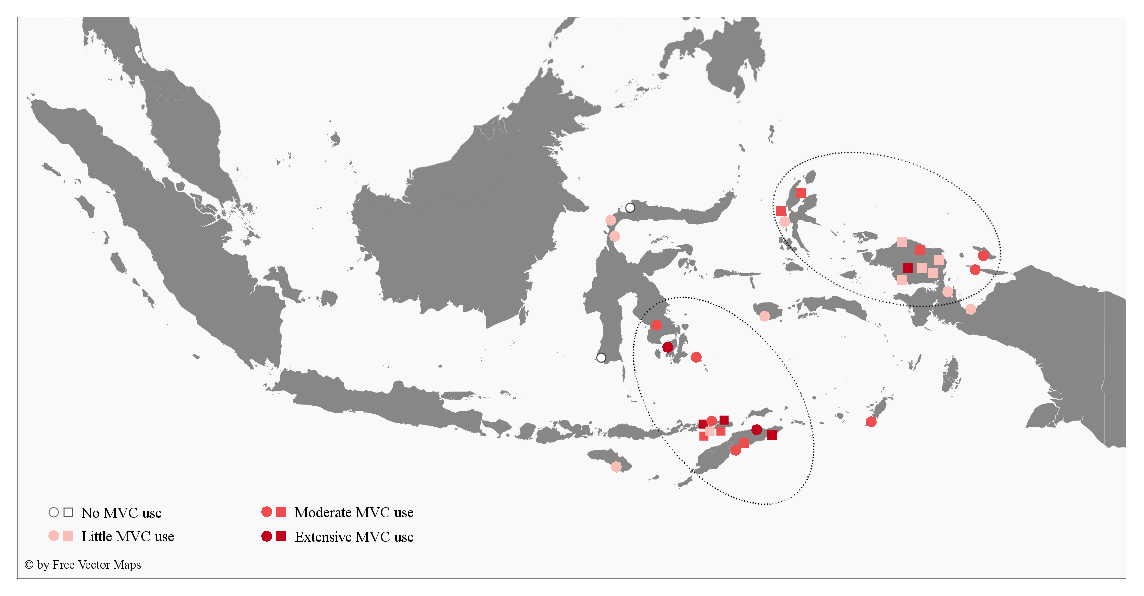
\includegraphics[width=\textwidth]{figures/Map_overview_klein_MVCuse_alt.eps}
\caption[Geographical distribution of linguistic profiles of MVC use across Eastern Indonesia]{Geographical distribution of linguistic profiles of MVC use across Eastern Indonesia. Languages are grouped into Austronesian (circles) and Papuan (squares). The colours designate the four linguistic profiles from Table \ref{table:profile_MVCuse}. Two Sulawesi languages, Totoli and Makassarese, have been added as outgroup examples, and are good candidates for the rank 0 profile. Potential core areas of MVC use are highlighted by dotted outlines.}\label{fig:map_profiles}
\end{sidewaysfigure}

Figure \ref{fig:map_profiles} is a visualisation of the geographical distribution of the different linguistic profiles across Eastern Indonesia. I also include two outgroup languages that I had given a cursory glance when compiling the sample (but dismissed due to a lack of attested MVCs). Both languages belong to the Western-Malayo-Polynesian branch of Austronesian, and are spoken in Sulawesi. Totoli, located on the Minahasa Peninsula at Tolitoli Bay in northern Sulawesi, was documented by another DoBeS language documentation project \citep{leto2012totoli}, and is related to Pendau and Tajio. Makassarese belongs to the South-Sulawesi branch of WMP and is spoken in Makassar and its vicinity on the tip of the South Peninsula \citep{jukes2005makassar, jukes2006makassarese}. For Totoli, I explored two pear story narrations from the Totoli corpus. For Makassarese I searched the publications including one appended text, but in both cases only very weak traces of MVC use could been found (basically pseudo-modal verb constructions involving \textsc{want} and \textsc{can} verbs, as well as a handful of examples that might be interpreted as motion-to-action). Thus, for the time being I tentatively assume that both Totoli and Makassarese constitute examples of the `no use' profile. If any dividing line is to be drawn between a Sprachbund area where the languages converge on using MVCs to at least some extent, and adjacent areas where MVCs play no or almost no role, it would in all likelihood run somewhere through Sulawesi.

From the distribution of rank II and rank III languages, we can identify two major `hotspots' of MVC use in EI: a southern core area appears to include the Timor-Alor-Pantar complex of languages, spoken on Timor and neighbouring islands. It is not only the Papuan TAP languages that conform to a high MVC use, but also the Austronesian neighbours like Waima'a and Tetun (and also, to a lesser degree, Alorese). This core area probably radiates out into south-eastern Sulawesi and includes the seafaring language communities of Muna and Tukang Besi with their long-standing history as traders \citep{donohue1999}. A second, though less pronounced, core area of MVC use can be seen stretching from the Bird's Head to Northern Halmahera, roughly covering the West Papuan zone of influence \textit{sensu} \citet{reesink2005west}. Here as well, we can observe that the Austronesian languages spoken in the same area are almost all classified as showing at least moderate MVC use. Taba is ranked lower, but still shows a sufficient amount of MVC use. The region between these MVC hotspots, the southern Moluccas, is clearly underrepresented in the sample, so that no real conclusion can be drawn. Yet judging from the two languages included in the sample it seems that the use of MVCs is indeed lower throughout this area. Recall that Selaru only yielded very few data points, so that the classification into rank II might be biased by a dearth of total observations. In general, it is evident that MVC use is specifically high in areas with Papuan presence. This could be taken to support the assumption that MVC formation is a Papuan trait rather than Austronesian, and that Austronesian languages with regular exposure to Papuan language communities might be prone to showing higher degrees of MVC use than more peripheral Austronesian languages.

\section{MVC formation: A view from discourse analysis} \label{sec:discourse}

A last issue to which I want to turn briefly is the prosody of MVCs as seen from a discourse perspective. I have argued in §\ref{sec:prosodic} and elsewhere that a strict match between syntactic units and prosodic units is implausible. Assuming that prosody cues the existence of grammatical constructions can only be a rough heuristic in order to delimit a certain set of observations thought to constitute a phenomenon of its own. I followed this heuristic while collating the EI data material, and assumed for the sake of crosslinguistic comparability that MVCs in EI are necessarily coherent prosodic units, with an unbroken f$_0$ contour and clear boundary signals to it.

This assumption only becomes problematic at the point where we start to infer syntactic boundaries from prosodic ones. In this section, I want to present some data, mostly from the two corpus languages Waima'a and Wooi, that illustrate the fallacy of such an inference, at least for the constructional families that correlate two event stages (that is, SREL and FJUX constructions). Data from published sources seldom contain contextual information. Examples of SVCs presented in grammatical descriptions are often chunks of utterances, IPs at best, that are stripped of their discourse relations, and isolated from their preceding units. Information on how such structures form as part of discourse practices is largely missing. Looking into natural speech data from Wooi and Waima'a suggests that such ``bare" examples from grammars and research papers may obscure the functions that MVCs possess in discourse development, and, as a consequence, their coming into being. Two-staged MVCs often do not appear to be formed and produced on the spot, but rather build up incrementally. Consider the following stretch of utterances from a Wooi explanatory describing the burning of, and planting of seedlings in, a forest garden.  

\ea \label{Wooi_gardening1}
\langinfo{Wooi}{Austronesian, SHWNG}{gardening\_exp1}\\
\ea 
\glll enuin da ve etiri ra kekavi \\
e-nuing ra ve e-iri ra $<$i$>$kakavi \\
\textsc{4}-burn until \textsc{purp} \textsc{4}-clear until $<$\textsc{3}\textsc{sg}$>$clean \\
\glft `It is burned for clearing (the spot) until it is empty' \\ 
\ex
\gll terus yo \\
then \textsc{fill} \\
\glft `then' \\ 
\ex
\glll a: tantanani \\
a: ta-tanang-i \\
\textsc{fill} \textsc{1}\textsc{pl}.\textsc{in}-plant-\textsc{obj}.\textsc{sg} \\
\glft `we plant it (with seedlings)' \\ 
\ex
\glll tatiri ra kekavi tantanani mara interi \\ 
ta-iri ra $<$i$>$kakavi ta-tanang-i mara interi \\
\textsc{1}\textsc{pl}.\textsc{in}-clear until $<$\textsc{3}\textsc{sg}$>$clean \textsc{1}\textsc{pl}.\textsc{in}-plant-\textsc{obj}.\textsc{sg} \textsc{top} then \\
\glft `we clear it until clean (and) plant it.'\\ 
\z
\z

The example consists of three utterances (and a regulatory filler), each separated by a final LH boundary tone and lengthening of the penultimate syllable. The first and the third intonation phrase each serve to establish one event. Both construals are in fact quite different. In the first IP an impersonal ``fourth person" subject is used. In the third IP, the speaker then shifts to a first person subject. The last IP finally combines the two events just established by wrapping it all up into what looks like a summary of the paragraph. While the verbs each come to stand at the very end of the first IPs, and articulation slows down at the lengthened segments, in the summarising IP they reappear in non-final position, with accelerated articulation speed and a reduction of word-final syllables. This directly reflects the difference in topicality. The event line is now well introduced and salient, so that the speaker can compress both event stages into one overall IP, and turn the whole sequence into a sentential topic marked by \textit{mara}. Figure \ref{fig:gardening_pitch} illustrates the prosodic properties of example (\ref{Wooi_gardening1}).

\begin{figure}
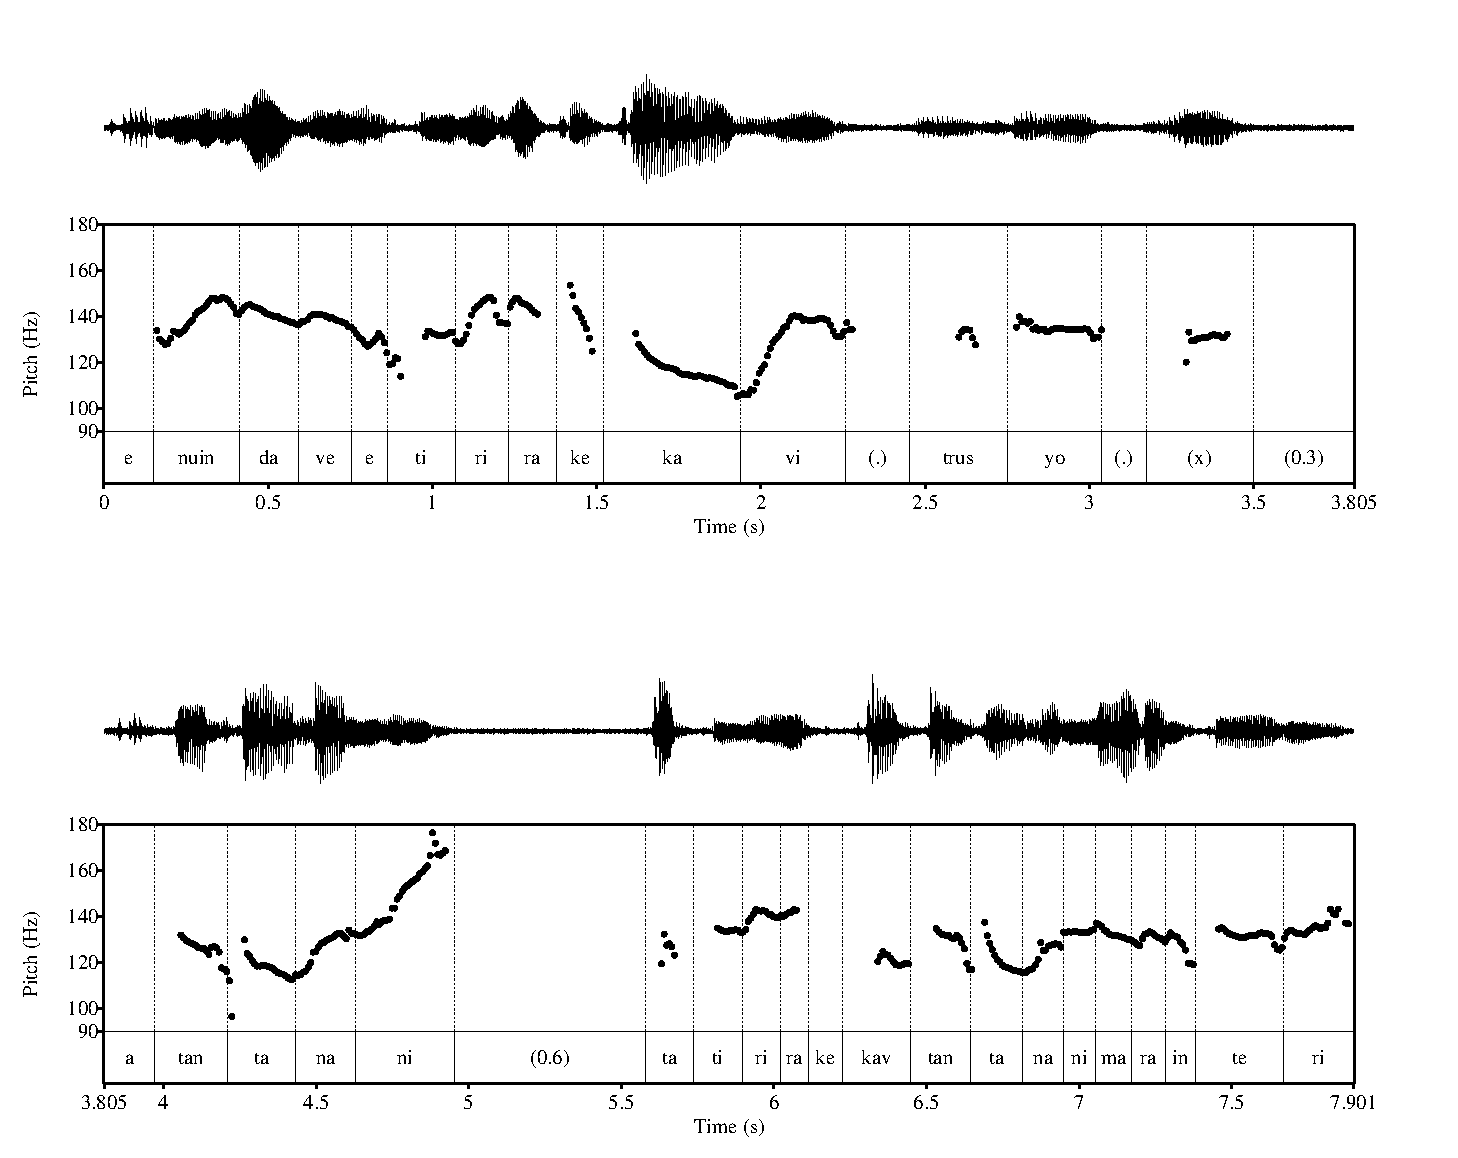
\includegraphics[width=1.2\textwidth]{figures/gardening1_burnplant.eps} 
\caption{F$_0$ contour of example (\ref{Wooi_gardening1})}\label{fig:gardening_pitch}
\end{figure}

Such incremental build-ups of compressed known information is in fact well known in Papuan linguistics. Papuan languages show strong preferences for a set of strategies that are crucial in discourse structuring and development \citep{devries2005towards, devries2006areal}. Three strategies are highly relevant in our context, and are found to actively shape the discourse structure in many EI languages (Papuan as well as Austronesian). 

Thematisation refers to the establishment of referents, locations and other discourse objects forming the inventory of participants for the text to follow \citep{heeschen1998eipo, devries2006areal}. Typical contexts of thematising are the beginning of texts, or at points where a break in the story-line occurs, and new discourse participants have to be introduced. Thematising often results in ``a paratactic series of thematic or setting constituents" \citep[814]{devries2006areal}. But thematisation is also evident from contexts  in which the story-line is progressing. In example (\ref{Wooi_gardening1}) from Wooi, the event construals established in the preceding IPs are not only compressed into a summarising IP, but the whole string of verbal constituents is marked as a sentential topic, which serves as the backdrop for the following utterances. The topic marker \textit{mara} in Wooi permits the wrapping of different verbal constituents into structures of unspecified length and complexity. It is thus not a topicaliser of clauses, but rather of sentences.

Distribution (of nominals) is a second major discourse strategy in Papuan languages also heavily shaping the way Papuan texts are organised \citep{devries2005towards, devries2006areal}. We have already seen examples of distributive strategies in EI languages. The Makalero verb system is a good example to begin with. Recall from §\ref{sec:nus} that Makalero prevents ditransitive argument configurations. A main verb provides one object slot which can be filled by a direct object argument, or by an adjunct complement \citep{huber2011}. Ditransitive argument frames are resolved by using multi-verb strings instead. As we have seen, \textit{mei} `take' has developed into a lightverb licensing further arguments into the event schema. Related strategies are found in other TAP languages, for instance in transfer constructions consisting of multi-verb strings \citep{klamer2012development}. Of course, Makalero is a rather extreme case where a discourse-based tendency has been conventionalised into grammatical rules. But, as \citet[813]{devries2006areal} put it, \begin{quote}[i]f there must be nominals, Papuan speakers [...] try to have no more than one nominal modifying the verb in the clause, and no more than one modifying element in the nominal phrase.\end{quote} This strategy results in structures that are rich in verbs, but where nominals are few, and sparsely distributed across MVCs, verb chains, and related mechanisms. Although distributive strategies are strongly associated with Papuan languages, Austronesian languages from the EI region show similar patterns. In isolating languages of Timor, such as Waima'a or Tetun Fehan, nominals are often dropped when participants are known or inferable from the discourse context, resulting in strings of verbs with only occasional occurrence of nominal expressions. Distributing nominals across utterances can also influence the formation of MVCs, as the following example from Wooi illustrates.

\ea \label{Wooi_leaf}
\langinfo{Wooi}{Austronesian, SHWNG}{MANTERA\_magic charms}\\
\ea
\glll ka: ariaung vati kori ma \\
kaynteri ariaung vati $\emptyset$-ko=i ma \\
next leaf \textsc{det}:\textsc{sg} \textsc{1}\textsc{sg}-take-\textsc{obj}.\textsc{sg} come \\
\glft `The leaf, I carry hither' \\ 
\ex
\glll kor ma honi ho botol \\
$\emptyset$-ko=i ma $\emptyset$-honi ho botol \\
\textsc{1}\textsc{sg}-take-\textsc{obj}.\textsc{sg} come \textsc{1}\textsc{sg}-fill \textsc{dir} bottle \\
\glft `I carry it hither and put it into a bottle.'\\
\z
\z

The short sequence of two utterances in (\ref{Wooi_leaf}) is part of an explanatory text on how to turn leaves from a particular tree into a magic charm. The leaf is established as a discourse participant in the first IP. \textit{Ariaung vati} is the first mention of the leaf in the text, and placed in preposed topic position before the verb\footnote{Topical fronting of nominals triggers the use of the resumptive clitic on the predicate.}. The second IP then serves to link the event depiction from the previous IP to the action coming next in the procedure. Instead of repeating the nominal, the leaf is referred to by use of the resumptive object clitic \textit{=i}, and another nominal, \textit{botol}, is used by the following verb to introduce a new participant. The MVC resulting from the linking process belongs to the motion-to-action construction. Note that it is only the two-stage SREL construction that is shaped by means of the distributive strategy. The component-relating MVC \textit{kori ma} is produced on the spot. This seems to be a general difference between CREL and SREL MVCs. I have never come across a single example of a component-relating construction that would emerge incrementally across two or more IPs.

Example (\ref{Wooi_leaf}) also illustrates another pervasive discourse strategy in the languages of New Guinea. I already mentioned that the content of the first IP is repeated in the second, and linked to the next predication. This pattern has come to be known as tail-head linkage, or recapitulative linkage in Papuan linguistics \citep{devries2005towards, devries2006areal}. Repeated structures such as the carrying from example (\ref{Wooi_leaf}) form the `tail' of the next clause (the `head'). Consider the paragraph in example (\ref{Korafe}) from Korafe, a Trans-New-Guinea language from PNG \citep{farr1999interface}.

\ea \label{Korafe}
\langinfo{Korafe}{Papuan}{\citealt[816]{devries2006areal}, quoted from \citealt[338]{farr1999interface}}\\
\ea
\gll vose bu jigh-ir-iri karaje mindi ambududuru-seri \\
descend.I get.I hold-remain-\textsc{sim}.\textsc{rls}.3\textsc{sg}.\textsc{ds} salt.water eat.I die.II-\textsc{dpst}.3\textsc{pl}.\textsc{fn} \\
\glft `It descended and held them while they drowned (lit. ate salt water and died).' \\ 
\ex
\gll amb-ero gi-do bebesuge-tiri eroru-seri \\
die.I-\textsc{seq}.\textsc{rls}.3\textsc{pl}.\textsc{ds} see.I-\textsc{seq}.\textsc{ss} open.up.\textsc{rdp}.I-\textsc{seq}.\textsc{rls}.3\textsc{sg}.\textsc{ds} arise.II-\textsc{dpst}.3\textsc{pl}.\textsc{fn} \\
\glft `Seeing that they had died, it opened out its tentacles and they floated up.' \\ 
\ex
\gll ere-do, feeghe viti-f-era \\ 
arise.I-\textsc{seq}.\textsc{ss} float.I ascend.I-come.\textsc{dur}-\textsc{seq}.\textsc{rls}.\textsc{pst}.3\textsc{pl}.\textsc{ss} \\
\glft `Their bodies arose, floated and came up and...' \\ 
\z
\z

Korafe is a clause-chaining language and employs suffixes on the medial verbs in order to facilitate subject tracking. Example (\ref{Korafe}) consists of three clause-chains. At the beginning of each new chain, the finite clause from the previous chain is repeated as the `tail' of the new chain, producing two cases of tail-head linkage. Cases of recapitulative linkage are also frequently found in natural speech data from the EI languages. Consider example (\ref{Waimaqa_dom2_22}) from Waima'a.

\ea \label{Waimaqa_dom2_22}
\langinfo{Waima'a}{Austronesian, CMP}{dom2\_kaben 22--3}\\
\ea
\glll kuandu laka is nan la basara \\
kuandu laka isi nani la basara \\
when go \textsc{ptl} perhaps \textsc{loc} market \\
\glft `When they go to the market,' \\ 
\ex
\gll kas nan basara wuo-ruo hita ini \\ 
go:\textsc{ptl} perhaps market \textsc{clf}-two find \textsc{recp} \\
\glft `going to the market the two would meet.'\\ 
\z
\z

As in the Wooi example above, the clause from the first intonation phrase is repeated as the tail of a tail-head linkage in the second IP. Although the adverb \textit{nan} and the nominal expression \textit{la basara} are not dropped in this case, we still see the formation of a motion-to-action MVC through repetition of known information from a previous IP. The verb complex \textit{laka is} is shortened to \textit{kas} in the second IP, just as we can expect with known information (mirroring the accelerated articulation rate and the dropping of final segments from example (\ref{Wooi_gardening1})). Recapitulative linkage is not limited to motion-to-action in EI languages, and can also produce longer series. Here is another example from Waima'a in which an initial motion stage is produced, but not repeated in the final MVC. 

\ea \label{Waimaqa_cuttwine}
\langinfo{Waima'a}{Austronesian, CMP}{Julio\_goat 26--9}\\
\ea
\gll laka bo \\
go about.to \\
\glft `They go and' \\
\ex
\gll rutu huko \\
cut k.o.plant \\
\glft `cut a kind of plant called ``Huko"' \\
\ex
\glll wuruo l'ele \\
wuo-ruo l'ele \\
\textsc{clf}-two spin \\
\glft `they twine a rope' \\
\ex
\glll rutu huko wuruo l'ele \\
rutu huko wuo-ruo l'ele \\
cut k.o.plant \textsc{clf}-two spin \\
\glft `they cut the Huko (to) twine a rope.'\\
\z
\z

Example (\ref{Waimaqa_cuttwine}) is already a little bit more elaborate than the strict tail-head pattern that we have seen in example (\ref{Korafe}) from Korafe. Instead of directly linking the cutting of Huko to the twining of the rope in the third IP, the action of twining the rope is established first. Only then, in the fourth IP, are both events linked together. This strategy is another instance of what we have seen in the introductory example from Wooi in (\ref{Wooi_gardening1}). The constituents of a paragraph are established one by one, followed by a final IP in which the most relevant parts are compressed and summarised (the going is not reiterated). \citet{heeschen1998eipo} describes elaborate summarising constructions from the Papuan language Eipo, spoken in the highlands of Indonesian Papua. As we can gather from the following example, summarising constructions in Eipo may build up across voluminous paragraphs.

\ea \label{eipo}
\langinfo{Eipo}{Papuan}{\citealt[308]{heeschen1998eipo}}\\
\ea
\gll kwalye deib-uk obora, wine bu-n-m-uk-buk, ore Sunum mereye oke di-n-m-uk-ak deib-uk obora, basam arye wine deib-uk obora, Sunum deib-uk. \\
banana put-3\textsc{sg}.\textsc{rpst} after now sit-\textsc{rep}-\textsc{dur}-3\textsc{sg}.\textsc{rpst}-when/\textsc{ds} and Sunum labour pain eat-\textsc{rep}-\textsc{dur}-3\textsc{sg}.\textsc{rpst}-at put-3\textsc{sg}.\textsc{rpst} after pig \textsc{sbj} now put-3\textsc{sg}.\textsc{rpst} after Sunum put-3\textsc{sg}.\textsc{rpst} \\
\glft `[...] She gave birth to the banana, and then, while she was sitting around, the pains of her labour for Sunum were consuming her, and there she gave birth to, the pig gave birth to, she gave birth to Sunum.' \\ 
\ex
\gll ninye deib-uk \\
Man put-3\textsc{sg}.\textsc{rpst} \\
\glft `She gave birth to Man.' \\ 
\ex
\gll ninye deib-uk obora: ``wirib-nama-n-do?" tenen bu-lam-uk-buk, basam ninye dei-am-uk \\ 
Man put-3\textsc{sg}.\textsc{rpst} after do/how-\textsc{nfut}-1\textsc{sg}-\textsc{q} think/\textsc{vn} sit-\textsc{hab}-3\textsc{sg}.\textsc{rpst}-\textsc{advrs} pig Man put-\textsc{perf}-3\textsc{sg}.\textsc{rpst} \\
\glft `And while she still gave birth to Man, and while she still thought: ``What shall I do?" (it happened that) the pig had given birth to Man.'\\ 
\z
\z

The paragraph from example (\ref{eipo}) recounts an ancestral myth about a female pig giving birth to Man. \citet[308]{heeschen1998eipo} remarks that 

\begin{quote}even simple SOV-clauses [...] have such a textual history and represent acts of summarizing. [...] The final SOV-clause summarizes the general content of the myth: the pig gives birth to somthing or someone, actually, it assembles the smaller units ``the pig gave birth to" and ``she gave birth to Man".\end{quote} 

In this case, the verbs of both smaller units are identical, so that no MVC follows from it. But the example serves to illustrate Eipo forms of summarising, and how the distribution of nominals may shape entire paragraphs. Such forms of summarising are also found in some of the EI languages.

The next example from Wooi shows another MVC formation over several IPs, produced by the elderly Wooi lady from the same recording as in example (\ref{Wooi_leaf}). Although clearly less comprehensive than the Eipo example above, the final IP summarises two event construals elaborated in four previous IPs. The resulting MVC in this case belongs to the position-action SREL. Notice that the locative PP \textit{na antureng repong} from the fourth IP is not repeated in the final MVC.

\ea 
\langinfo{Wooi}{Austronesian, SHWNG}{MANTERA\_magic\_charms 22--6}\\
\ea
\glll trus tera mainte \\
trus $\emptyset$-tera mainte \\
next \textsc{1}\textsc{sg}-stand then \\
\glft `Then I stand (up) and'\\ 
\ex
\glll ruva vara to wirey ra \\
$\emptyset$-ruva vara to wirey ra \\
\textsc{1}\textsc{sg}-lift hand \textsc{dir} forest go \\
\glft `I raise my hands up towards the forest'\\ 
\ex
\glll ruva vara to wirey \\
$\emptyset$-ruva vara to wirey \\
\textsc{1}\textsc{sg}-lift hand \textsc{dir} forest \\
\glft `I raise my hands towards the forest'\\ 
\ex
\glll te na antureng repong mainte \\
$\emptyset$-tera na antureng re-pong mainte \\
\textsc{1}\textsc{sg}-stand \textsc{loc} door \textsc{pos}-front then \\
\glft `I stand at the front door'\\ 
\ex
\glll tera ruva vara to wirey \\
$\emptyset$-tera $\emptyset$-ruva vara to wirey \\
\textsc{1}\textsc{sg}-stand \textsc{1}\textsc{sg}-lift hand \textsc{dir} forest \\
\glft `I stand (and) raise up my hands toward the forest.'\\ 
\z
\z

Again we can see here that the structure is slightly different from tail-head-linkage. We may therefore assume that recapitulative linkage in a rather broad sense includes both forms of summarizing, and forms of tail-head linkage, and both strategies are found in the corpus languages Wooi and Waima'a. We may, on the basis of these data, assume that we might also find these discourse strategies in other EI languages. Detecting them, however, is more difficult in published data sources than in comprehensive natural speech corpora as the interpretation of potential cases often hinges on small details, such as the placement of commas in appended texts suggesting intonation breaks between two IPs.

Summing up this section, we have seen that, if the discourse context is taken into consideration, two-stage MVCs do not just appear out of thin air, but may be carefully built up across several IPs. The driving factor behind such MVC formation in the EI region is a general preference of languages from New Guinea and beyond to distribute nominal information across verb series, and to link known information with new information in specific ways. This indicates very clearly that prosodic segmentation should not be assumed to accurately demarcate the syntactic boundaries of grammatical constructions. Instead, prosody provides a means of packaging information into parsable chunks. Linguistic research into multi-verb strings has up to now been mainly occupied with finding evidence for coherent units. As a detailed discourse analysis of MVCs in Eastern Indonesian languages is beyond the scope of this book, this section could only present an initial exploration of the hypothesis that some MVC types may come into being by aggregation rather than by coherence. Assuming such a discourse perspective would certainly provide new insights into the formation, distribution and function of MVCs, and may even help reject some of the hypotheses (like the monoclausality conundrum) that have been so fondly inherited from the debate on verb serialisation.

\section{Concluding remarks} \label{sec:concluding}

In this book, I have reviewed a data sample from 32 Eastern Indonesian languages with regard to the extent to which they express event construals of different sorts in multi-verb constructions. An overall 2146 instances of putative MVCs were collated and annotated for both formal and semantic parameters. The analysis of this sample has led to the formulation of five basic hypotheses, as introduced in Chapter \ref{ch:introduction}, and repeated here for the sake of convenience:

\begin{itemize}
\item \textbf{\#H1:} Although the morphosyntactic make-up of MVCs in EI is remarkably similar across different construction types, these MVCs are constructed through different techniques (mentioned below in H2)
\item \textbf{\#H2:} Verbal interaction in MVC formation involves three principle techniques at the clausal level: merging (of features), modification and staging (alignment of spatiotemporally distinct stages)
\item \textbf{\#H3:} The different techniques of MVC formation are based on a layered structure of event conception, each technique being associated with a particular level of the event schema
\item \textbf{\#H4:} Some MVC types may be embedded into a constructional slot of another MVC resulting in stacked MVCs
\item \textbf{\#H5:} Not all EI languages use all techniques. Differences in the use of MVC patterns indicate different linguistic subareas or diffusion zones of grammatical traits. MVC use radiates out from two hotspots of MVC innovation: the Timor-Alor-Pantar and the Bird's Head region, respectively.
\end{itemize}

In Chapter \ref{ch:area}, I argued that `linguistic Wallacea' can be supported both by evidence from genealogical descendance of the languages from an Austronesian or non-Austronesian (Papuan) origin as well as from typological characteristics of their grammatical systems. Discussing verb-related properties of the languages included in the EI sample revealed that they have strikingly similar characteristics (take person-marking systems and their limits to cross-reference O arguments), and that they are quite different at the same time (for instance, by organising function-argument interaction in symmetrical voice systems in Sulawesi languages, or without diathesis alternations to the east of the area). Based on these findings, the languages of Eastern Indonesia have been grouped into four subareas for which different degrees of, and exposure to, MVC formation could be expected. 

In Chapter \ref{ch:theory} I presented a review of the literature on verb serialisation. The debate on serialisation has been ongoing for several decades, and has led to a staggering amount of assumptions that are unsuitable for thorough testing, and, consequently, to a profusion of new criteria to which `real' SVCs ought to conform. Based on a critical assessment of defining features from different linguistic layers (grammar, lexicon, prosody, cognition), I introduced as an alternative the concept of \textit{multi-verb construction}, which at the end of Chapter \ref{ch:theory} was provided with a preliminary definition. Basically following Ameka's use of the term, MVCs are assumed to contain two or more verb-like elements predicating lexical content and being subcategorised for a certain argument frame, bearing no formal signs of dependency or hierarchical ranking, lacking a linking element, occurring within a coherent prosodic unit, and entailing a continuous temporal development without any in-between time lag. 

From the literature review in Chapter \ref{ch:theory}, three morphosyntactic properties were isolated that could be tested on published data. The pioneering study on verb serialisation in Eastern Indonesia \citep{vanstaden2008serial} relied upon portmanteau concepts combining the features headedness, referentiality, and contiguity into four different categories. These feature bundles were, in Chapter \ref{ch:gram}, disentangled and tested separately. The results suggested that variation in these features is neither associated with genetic affiliation of the languages nor with specific areal subgroups. Prototypical MVCs from the EI area were shown to have shared subjects (referentiality pattern ``S"), the same amount of inflection on both (all) verbal heads (headedness pattern ``B"), and the verbs placed in contiguous sequence (contiguity pattern ``C"). The finding from \citet[48]{vanstaden2008serial} that ``independent serialisation is by far the most commonly found type" could thus be reproduced with a larger sample. However, it became clear that, as all languages basically support all coding options (except for the headedness parameter which cannot be assessed in languages with unreliable morphology), the morphosyntactic make-up of MVCs in general does not reveal very much about the way MVCs are formed, distributed, and used.

As a consequence, in Chapter \ref{ch:sem} I drew on semantic approaches to explain the basic mechanisms underlying MVC formation. Semantic approaches in verb serialisation have often resorted to making statements about events, subevents and so on, without indicating how to identify them. The discussion in Chapter \ref{ch:sem} sets out from the assumption that linguistic event schemas are construed at levels of different complexity, and are associated with particular grammatical structures. The bottommost event schema is associated with lexical predicators (typically verbs), representing shared experience of some recurring real world event patterns reduced into linguistic form. Events at the lexeme-level were called LLEs. I proposed to assess the key components of LLEs by resorting to two approaches from formal semantics. Davidsonian event arguments were explored as a way to model the spatiotemporal characterists of linguistic event schemas. As each dynamic verb licenses its own event argument, several kinds of interaction between the event arguments of different verbs are possible: they may either merge, or remain independent. I referred to the latter case as staging of event arguments. Stative verbs (as well as certain groups of non-prototypical dynamic verbs), on the other hand, were assumed to not contribute a spatiotemporally defined event argument. Instead, the use of such verbs in MVCs typically results in their taking over the event schema of a dynamic matrix verb. This process was called modification. 

A second approach to detecting meaningful sublexical structure was pursued with a lexical decomposition model, based on \citet{van1997syntax}, and supplemented with two further predicate functions, \textbf{move'} and \textbf{say'}, to model motion verbs and speech verbs, respectively. Lexical decomposition was then applied to distinguish between merging on the one hand (where verbs from the same classes would merge part of their sublexical structure, paralleling the merging of event arguments), and modification and staging on the other hand, where no merging of sublexical features takes place. As verbs aggregate to strings, more complex event schemas were assumed to emerge at higher levels. At the predicate level, predicate-level events (PLE) were defined. Finally, at the next higher level, clause-level events (CLE) form. The distinction between PLEs and CLEs is supported by differences between merging constructions and staging constructions. It is only with the latter that shared arguments may be assigned different syntactic functions (for instance, in \textsc{cause-result} MVCs) or different semantic roles (recall example (\ref{Hatam6465}) from §\ref{sec:mvc-types} showing a motion-to-action MVC with a verb of sleeping in the action slot). The chapter closed by discussing one possible way of modelling the different techniques of MVC formation by using feature percolation trees.

A central conclusion from this study is that MVC formation in Eastern Indonesia is by no means a unified process, but rather consists of a multitude of different constructions. To force on this pattern diversity a single concept such as `verb serialisation' that is laden with a heavy rucksack of theoretical presuppositions, is therefore not helpful. Quite the contrary, it might even conceal the basic mechanisms at work in MVCs. In Chapter \ref{ch:constructions}, I classified the retrieved constructions into four constructional families, each one shaped by a specific technique of MVC formation, as laid out in Chapter \ref{ch:sem}. Component-relating constructions are composed of verbs with identical sublexical structure. Verbs in modifying constructions lack this sublexical identity. Rather, a modifier verb combines with a matrix verb. Both CREL and MOD constructions have been found to consist of a simple event structure. This is a stark contrast to stage-relating and free juxtaposition constructions which both have complex event structures organised into a succession of event stages. While FJUX constructions appear to possess but a few restrictions, and their constituent parts act rather independently, SREL constructions operate over conventionalised sequences of stages defined by restricted host classes like motion verbs, posture verbs, or verbs of handling. In many EI languages, SREL constructions exhibit specific grammatical properties, or restrictions, which seem to set them apart from free juxtaposition. However, as indicated by the findings from the previous section, SREL and FJUX constructions do not appear to be so different after all. Both may be shaped by the same pragmatic strategies, incrementally aggregating verb series across several intonation phrases. MVCs of this kind are not necessarily generated \textit{ad hoc}, but may rather emerge as the result of shifts in the information-structural encoding of constituents. Those collocations that are particularily frequent, and reflect culturally salient event concatenations, may become conventionalised over time, giving rise to specific multi-verb templates such as motion-to-action or cause-result in Eastern Indonesia, and possibly to even more elaborate ones in languages like Kalam.

In terms of MVC use and distribution across Eastern Indonesia, this study has shown that the formation of MVCs is likely to be a general trait found in most, if not all, languages throughout linguistic Wallacea. All 32 languages make use of at least a fraction of the constructions attested for the area as a whole. The distribution of constructions, however, is not even. While genetic descendance seems to be of minor importance, the four subareas were seen to differ as to which constructions are attested. While MOD constructions and FJUX constructions can be observed in every subgroup, CREL and SREL constructions are less well attested in the Sulawesi subgroup, with some constructions being not attested at all. Some SRELs are also hardly attested in the Maluku subgroup. In this chapter, I calculated a diversity score (D-score) for each language which indicates the amount of constructional diversity. The D-score showed that Abui and Makalero from the Nusa Tenggara group, Muna from Sulawesi, and Maybrat from Western Papua display the greatest MVC diversity. 

The D-score was then compared to the amount of stacked MVCs per language. Stacked MVCs are complex combinations of two or even more MVCs. Decomposing such MVCs leads to the detection of hierarchical structures. As we have seen, recursion in MVCs always takes place at the `edge' of a constructional string, making it difficult to ascertain the existence of hierarchies (and ruling out paratactic series). A look at Lao in mainland South-East Asia, however, revealed multi-verb structures that are strikingly similar to the cases of stacked MVCs that I described for the EI area. In both cases, complex verb concatenations are best analysed as sets of binary verb pairs nested into the slots of higher-order MVCs. However, not all languages of EI produce stacked MVCs to the same extent. In order to use the amount of hierarchical MVCs as another indicator of overall MVC use, I calculated the C-score, indexing the number of stacked MVCs in relation to the total number of MVC observations.

Both the D-score and the C-score were then combined into four different profiles of MVC use. Rank 0 languages make no use of MVCs at all (such languages were not part of the sample, but the Austronesian languages Totoli and Makassarese were tentatively identified as candidates). Rank I languages show little MVC use, and 13 languages were associated with this profile. Rank II languages show moderate MVC use, and 15 such languages were identified in the sample. Finally, rank III languages show extensive use of MVC, both by using many different constructions, and displaying a high amount of constructional complexity in MVCs. Six languages were labelled as rank III languages: Muna, Abui, Makalero, Teiwa, Waima'a, and Maybrat. Except for the first and the last one, all these languages belong to the Nusa Tenggara group. A geographical analysis of where the linguistic profiles occur shows that Eastern Indonesia appears to have two core areas of MVC use. The western hotspot comprises the TAP area on Timor and its vicinity, and possibly stretches up to south-east Sulawesi. A second, though weaker, hotspot can be identified stretching from the Bird's Head to northern Halmahera. These core areas of MVC use contrast with more peripheral areas, such as northern Sulawesi or the southern Moluccas. At present, this suggests that high MVC use clusters around the central zones of Papuan presence in EI, but more data would be needed in order to confirm these patterns.

\section{Avenues for future research}

This book was based on a literature survey. By collating material from grammars, research papers and language documentation databases, the aim was to present an areal account of MVC use in Eastern Indonesia, to make the grammatical descriptions of MVCs from individual languages accessible, and to provide a framework which would allow for cross-linguistic comparisons. The limits that are associated with such a literature survey prevented a thorough testing of hypotheses at some points, so that the conclusions arrived at in the previous section, can only be tentative ones. It is hoped that the tendencies and implications found so far will be scrutinised in future work on MVCs in Eastern Indonesia and beyond. At this point, I would like to point out some research directions which it might be worth exploring further..

I have shown that MVC usage can be a further diagnostic to help determine the existence of a Wallacean Sprachbund area in Eastern Indonesia. The exact limits of MVC use, however, would need to be tested further by adding more languages, and also more data material, to the tentative picture presented in §\ref{sec:profile_use}. Two points are of major interest here. First, it is important to further assess and determine the outer limits of linguistic Wallacea by looking into languages from Sulawesi on the one hand, and into languages spoken in the eastern Cenderawasih Bay area, as well as on Bomberai peninsula, on the other.  Second, we have seen that the Moluccan subarea still consists of many white spots, and the few languages investigated indicate only little MVC use (cf. Figure \ref{fig:map_profiles}). Looking into more languages in this subarea would clearly be helpful with regard to the assumption of two separate central zones of MVC innovation in Eastern Indonesia.

A second promising direction would be to follow up on my tentative comparison between MVC formation in EI and MVCs from Lao. While there seems to be a dearth of MVC languages in Western Indonesia, there are other linguistic areas nearby with reported MVC use. To the east, we find a wealth of Papuan language families on mainland New Guinea that attest to different kinds of multi-verb strategies, among others systems of verb chaining. For instance, research into Yali, a Papuan language spoken in the Western Highlands of Indonesian Papua, has shown that clause-chaining and serialising strategies may co-occur \citep{riesberg2013}. The exact limits as to which concepts are expressed by multi-verb strategies are yet to be drawn, and may help to further our understanding of MVC formation in Eastern Indonesia. And to the west, beyond the Western Austronesian `bubble' of non-MVC languages, we find the Tai-Kadai and the Hmong-Mien language families, both featuring descriptions of MVCs. For instance, \citet{jarkey2010cotemporal} presents an analysis of `co-temporal' SVCs from White Hmong, and discusses constructions that are remarkably similar to many of the MVCs discussed in Chapter \ref{ch:constructions}. A comparison of Eastern Indonesian MVCs with multi-verb strings found in the languages of mainland South-East Asia might unearth common patterns of use that may be shared over much greater distances than just within the horizons of linguistic Wallacea.

Finally, and perhaps most interestingly, the semantic analysis of MVCs, as outlined in Chapter \ref{ch:sem}, has revealed four different formation techniques. As we have seen in §\ref{sec:discourse} above, it is not only by coherence that MVCs come into being (as much recent work has explicitly or implicitly assumed), but also by aggregation on the discourse level. Seen this way, the findings from this book suggest an intermediate position between the two outer poles of coherence and composition, as briefly introduced in §\ref{sec:coherence}. Research into larger samples could determine the extent to which aggregation driven by pragmatic strategies contributes to the formation and use of MVCs. It is in this context that the role of prosody in MVC encoding should be critically (re)examined. The underlying techniques of MVC formation, giving rise to single-stage and two-stage MVC construals, as well as the basic constraints associated with them, may provide valuable insights into the landscape of MVCs in Eastern Indonesia, and perhaps beyond.
